\documentclass{article}

  % packages
    % basic stuff for rendering math
    \usepackage[letterpaper, top=1in, bottom=1in, left=1in, right=1in]{geometry}
    \usepackage[utf8]{inputenc}
    \usepackage[english]{babel}
    \usepackage{amsmath} 
    \usepackage{amssymb}
    % \usepackage{amsthm}

    % extra math symbols and utilities
    \usepackage{mathtools}        % for extra stuff like \coloneqq
    \usepackage{mathrsfs}         % for extra stuff like \mathsrc{}
    \usepackage{centernot}        % for the centernot arrow 
    \usepackage{bm}               % for better boldsymbol/mathbf 
    \usepackage{enumitem}         % better control over enumerate, itemize
    \usepackage{hyperref}         % for hypertext linking
    \usepackage{fancyvrb}          % for better verbatim environments
    \usepackage{newverbs}         % for texttt{}
    \usepackage{xcolor}           % for colored text 
    \usepackage{listings}         % to include code
    \usepackage{lstautogobble}    % helper package for code
    \usepackage{parcolumns}       % for side by side columns for two column code
    

    % page layout
    \usepackage{fancyhdr}         % for headers and footers 
    \usepackage{lastpage}         % to include last page number in footer 
    \usepackage{parskip}          % for no indentation and space between paragraphs    
    \usepackage[T1]{fontenc}      % to include \textbackslash
    \usepackage{footnote}
    \usepackage{etoolbox}

    % for custom environments
    \usepackage{tcolorbox}        % for better colored boxes in custom environments
    \tcbuselibrary{breakable}     % to allow tcolorboxes to break across pages

    % figures
    \usepackage{pgfplots}
    \pgfplotsset{compat=1.18}
    \usepackage{float}            % for [H] figure placement
    \usepackage{tikz}
    \usepackage{tikz-cd}
    \usepackage{circuitikz}
    \usetikzlibrary{arrows}
    \usetikzlibrary{positioning}
    \usetikzlibrary{calc}
    \usepackage{graphicx}
    \usepackage{algorithmic}
    \usepackage{caption} 
    \usepackage{subcaption}
    \captionsetup{font=small}

    % for tabular stuff 
    \usepackage{dcolumn}

    \usepackage[nottoc]{tocbibind}
    \pdfsuppresswarningpagegroup=1
    \hfuzz=5.002pt                % ignore overfull hbox badness warnings below this limit

  % New and replaced operators
    \DeclareMathOperator{\Tr}{Tr}
    \DeclareMathOperator{\Sym}{Sym}
    \DeclareMathOperator{\Span}{span}
    \DeclareMathOperator{\std}{std}
    \DeclareMathOperator{\Cov}{Cov}
    \DeclareMathOperator{\Var}{Var}
    \DeclareMathOperator{\Corr}{Corr}
    \DeclareMathOperator{\pos}{pos}
    \DeclareMathOperator{\im}{Im}
    \DeclareMathOperator*{\argmin}{\arg\!\min}
    \DeclareMathOperator*{\argmax}{\arg\!\max}
    \newcommand{\ket}[1]{\ensuremath{\left|#1\right\rangle}}
    \newcommand{\bra}[1]{\ensuremath{\left\langle#1\right|}}
    \newcommand{\braket}[2]{\langle #1 | #2 \rangle}
    \newcommand{\qed}{\hfill$\blacksquare$}     % I like QED squares to be black

  % Custom Environments
    \newtcolorbox[auto counter, number within=section]{question}[1][]
    {
      colframe = orange!25,
      colback  = orange!10,
      coltitle = orange!20!black,  
      breakable, 
      title = \textbf{Question \thetcbcounter ~(#1)}
    }

    \newtcolorbox[auto counter, number within=section]{exercise}[1][]
    {
      colframe = teal!25,
      colback  = teal!10,
      coltitle = teal!20!black,  
      breakable, 
      title = \textbf{Exercise \thetcbcounter ~(#1)}
    }
    \newtcolorbox[auto counter, number within=section]{solution}[1][]
    {
      colframe = violet!25,
      colback  = violet!10,
      coltitle = violet!20!black,  
      breakable, 
      title = \textbf{Solution \thetcbcounter}
    }
    \newtcolorbox[auto counter, number within=section]{lemma}[1][]
    {
      colframe = red!25,
      colback  = red!10,
      coltitle = red!20!black,  
      breakable, 
      title = \textbf{Lemma \thetcbcounter ~(#1)}
    }
    \newtcolorbox[auto counter, number within=section]{theorem}[1][]
    {
      colframe = red!25,
      colback  = red!10,
      coltitle = red!20!black,  
      breakable, 
      title = \textbf{Theorem \thetcbcounter ~(#1)}
    } 
    \newtcolorbox[auto counter, number within=section]{proposition}[1][]
    {
      colframe = red!25,
      colback  = red!10,
      coltitle = red!20!black,  
      breakable, 
      title = \textbf{Proposition \thetcbcounter ~(#1)}
    } 
    \newtcolorbox[auto counter, number within=section]{corollary}[1][]
    {
      colframe = red!25,
      colback  = red!10,
      coltitle = red!20!black,  
      breakable, 
      title = \textbf{Corollary \thetcbcounter ~(#1)}
    } 
    \newtcolorbox[auto counter, number within=section]{proof}[1][]
    {
      colframe = orange!25,
      colback  = orange!10,
      coltitle = orange!20!black,  
      breakable, 
      title = \textbf{Proof. }
    } 
    \newtcolorbox[auto counter, number within=section]{definition}[1][]
    {
      colframe = yellow!25,
      colback  = yellow!10,
      coltitle = yellow!20!black,  
      breakable, 
      title = \textbf{Definition \thetcbcounter ~(#1)}
    } 
    \newtcolorbox[auto counter, number within=section]{example}[1][]
    {
      colframe = blue!25,
      colback  = blue!10,
      coltitle = blue!20!black,  
      breakable, 
      title = \textbf{Example \thetcbcounter ~(#1)}
    } 
    \newtcolorbox[auto counter, number within=section]{code}[1][]
    {
      colframe = green!25,
      colback  = green!10,
      coltitle = green!20!black,  
      breakable, 
      title = \textbf{Code \thetcbcounter ~(#1)}
    } 
    \newtcolorbox[auto counter, number within=section]{algo}[1][]
    {
      colframe = green!25,
      colback  = green!10,
      coltitle = green!20!black,  
      breakable, 
      title = \textbf{Algorithm \thetcbcounter ~(#1)}
    } 

    \BeforeBeginEnvironment{example}{\savenotes}
    \AfterEndEnvironment{example}{\spewnotes}
    \BeforeBeginEnvironment{lemma}{\savenotes}
    \AfterEndEnvironment{lemma}{\spewnotes}
    \BeforeBeginEnvironment{theorem}{\savenotes}
    \AfterEndEnvironment{theorem}{\spewnotes}
    \BeforeBeginEnvironment{corollary}{\savenotes}
    \AfterEndEnvironment{corollary}{\spewnotes}
    \BeforeBeginEnvironment{proposition}{\savenotes}
    \AfterEndEnvironment{proposition}{\spewnotes}
    \BeforeBeginEnvironment{definition}{\savenotes}
    \AfterEndEnvironment{definition}{\spewnotes}
    \BeforeBeginEnvironment{exercise}{\savenotes}
    \AfterEndEnvironment{exercise}{\spewnotes}
    \BeforeBeginEnvironment{proof}{\savenotes}
    \AfterEndEnvironment{proof}{\spewnotes}
    \BeforeBeginEnvironment{solution}{\savenotes}
    \AfterEndEnvironment{solution}{\spewnotes}
    \BeforeBeginEnvironment{question}{\savenotes}
    \AfterEndEnvironment{question}{\spewnotes}
    \BeforeBeginEnvironment{code}{\savenotes}
    \AfterEndEnvironment{code}{\spewnotes}
    \BeforeBeginEnvironment{algo}{\savenotes}
    \AfterEndEnvironment{algo}{\spewnotes}

    \definecolor{dkgreen}{rgb}{0,0.6,0}
    \definecolor{gray}{rgb}{0.5,0.5,0.5}
    \definecolor{mauve}{rgb}{0.58,0,0.82}
    \definecolor{darkblue}{rgb}{0,0,139}
    \definecolor{lightgray}{gray}{0.93}
    \renewcommand{\algorithmiccomment}[1]{\hfill$\triangleright$\textcolor{blue}{#1}}

    % default options for listings (for code)
    \lstset{
      autogobble,
      frame=ltbr,
      language=Python,
      aboveskip=3mm,
      belowskip=3mm,
      showstringspaces=false,
      columns=fullflexible,
      keepspaces=true,
      basicstyle={\small\ttfamily},
      numbers=left,
      firstnumber=1,                        % start line number at 1
      numberstyle=\tiny\color{gray},
      keywordstyle=\color{blue},
      commentstyle=\color{dkgreen},
      stringstyle=\color{mauve},
      backgroundcolor=\color{lightgray}, 
      breaklines=true,                      % break lines
      breakatwhitespace=true,
      tabsize=3, 
      xleftmargin=2em, 
      framexleftmargin=1.5em, 
      stepnumber=1
    }

  % Page style
    \pagestyle{fancy}
    \fancyhead[L]{Point Set Topology}
    \fancyhead[C]{Muchang Bahng}
    \fancyhead[R]{Fall 2024} 
    \fancyfoot[C]{\thepage / \pageref{LastPage}}
    \renewcommand{\footrulewidth}{0.4pt}          % the footer line should be 0.4pt wide
    \renewcommand{\thispagestyle}[1]{}  % needed to include headers in title page

\begin{document}

\title{Point Set Topology}
\author{Muchang Bahng}
\date{Spring 2025}

\maketitle
\tableofcontents
\pagebreak

  Given a set, what are some fundamental structures that you can put on a set? We can first talk about relations, such as ordering, or functions, such as a norm or a distance. These are constructed as subsets of a Cartesian product of finite $X$'s. Another structure on set $X$ is to define a set of subsets $\mathscr{T} \subset 2^X$ that allow us to interpret how certain elements of a set are ``nearby'' each other without the notion of a metric.\footnote{In ZFC set theory, a topology may be more fundamental in the sense that it is a subset of the power set, while the other structures are subsets of a Cartesian product, which itself is a construction from the power set.} This set of subsets is called a \textit{topology}, with its elements being \textit{open sets}. So how do you define such a thing? Well intuitively, given two elements $x, y \in X$, if there exists two disjoint open sets $U_1, U_2$ such that $x \in U_1$ and $y \in U_2$, then we can \textit{distinguish} these points in such a way. If this is true for all points in $X$, then this gives us a nice \textit{Hausdorff} property to work with. If there exists no open sets that can do this, then $x$ and $y$, although distinct in $X$, may be \textit{indistinguishable} in the topological sense. 
  
  If this notion of nearness can be rigorously defined, we may be able to characterize the elements and subsets of $X$. One nice notion is the concept of \textit{limit points} which asks whether $x$ is ``infinitesimally close'' to a certain set. This allows us to define limits without the notion of a metric, and with this foundation we build the notion of continuity.    

  A trivial way to construct such a topology is to take the power set $2^X$ itself. However, this may be ``too big'' in a sense that no interesting properties can be deduced. But this doesn't mean we can take any subset of $2^X$. We compromise by defining topologies to be a subset of $2^X$ with certain properties, which we will mention in the next section. 

\section{Topologies} 

  \subsection{Open Sets} 

    \begin{definition}[Topology]
      Let $X$ be a set and $\mathscr{T}$ be a family of subsets of $X$. Then $\mathscr{T}$ is a \textbf{topology} on $X$\footnote{I will use script letters to denote topologies and capital letters to denote sets.} if it satisfies the following properties. 
      \begin{enumerate}
        \item \textit{Contains Empty and Whole Set}: 
        \begin{equation}
          \emptyset, X \in \mathscr{T}
        \end{equation}

        \item \textit{Closure Under Union}. If $\{U_\alpha\}_{\alpha \in A}$ is a class of sets in $\mathscr{T}$, then 
        \begin{equation}
          \bigcup_{\alpha \in A} U_\alpha \in \mathscr{T}
        \end{equation}

        \item \textit{Closure Under Finite Intersection}: If $U_1, \ldots, U_n$ is a finite class of sets in $\mathscr{T}$, then 
        \begin{equation}
         \bigcap_{i=1}^{n} U_i \in \mathscr{T}
        \end{equation}
      \end{enumerate}
      A \textbf{topological space} is denoted $(X, \mathscr{T})$. 
    \end{definition}

    This leads to the most general definition of an open set. 

    \begin{definition}[Open Set]
      The elements of $\mathscr{T}$ are called \textbf{open sets} in $X$.\footnote{As implied from the definition of a topology, the arbitrary union and finite intersection of any number of open sets is an open set.} An open set $U$ which contains a point $x$ is called an \textbf{open neighborhood} of $x$, denoted $U_x$. 
    \end{definition}

    Note that an open set doesn't really mean anything without talking about with respect to its topology. 

    Note that we restrict property 3 to be a \textbf{finite} intersection because if we don't, the open ball topology on $\mathbb{R}$ would imply that 
    \begin{equation}
      \bigcap_{i = 1}^{\infty} \Big( - \frac{1}{i}, \frac{1}{i} \Big) = 0
    \end{equation}
    is an open set $\implies$ all points are open sets too, which can be troublesome for later purposes. 

    \begin{example}[Topologies of a Set of Cardinality 3]
      There are a total of 29 topologies that we can construct on $\{1, 2, 3\}$. Two such examples are 
      \begin{enumerate}
        \item $\{\emptyset, \{1, 2\}, \{1, 2, 3\}\}$ 
        \item $\{\emptyset, 3, \{2, 3\}, \{1, 2, 3\}\}$
      \end{enumerate}
    \end{example} 

    \begin{theorem}[Obvious Topologies]
      Given a set $X$, 
      \begin{enumerate}
        \item $2^X$ is a topology, called the \textbf{discrete topology}. 
        \item $\{\emptyset, X \}$ is a topology, called the \textbf{indiscrete topology}. 
      \end{enumerate}
    \end{theorem}
    \begin{proof}
      Listed. 
      \begin{enumerate}
        \item The first property is trivially proven. From the theorems of set theory, $U_\alpha \subset X \implies \cup U_\alpha \subset X \implies \cup U_\alpha \in 2^X$. Finally the same logic holds for intersection as well. 
        \item The first property is trivially proven. We can check for the 4 combinations of unions and intersections and see that they all result in either $\emptyset$ or $X$. 
      \end{enumerate}
    \end{proof}

    Note that we don't need to have any structure (e.g. order, metric, measure) on our set $X$ to define a topology. Two trivial examples were shown above, but there are some interesting ones. 

    \begin{theorem}[Cofinite Topology]
      Given a set $X$, the set of all subsets of form 
      \begin{equation}
        X \setminus \{\text{any finite collection of points $a_{i}'s$}\}
      \end{equation}
      is a topology, called the \textbf{cofinite topology} or the \textbf{finite complement topology}. 
    \end{theorem}
    \begin{proof}
      
    \end{proof}

    For common sets like $\mathbb{R}^n$, which has an inner product, or $\mathbb{Q}$, which has an order, it is easy to build these topologies with set-builder notation. Consider the following. 

    \begin{theorem}[Metric Topology]
      Given a metric space $(X, d)$, let us denote the \textbf{metric topology}, or \textbf{open-ball topology}, as the set of subsets $U$ satisfying the property that for all $x \in U$, there exists a positive $r \in \mathbb{R}$ such that $B(x, r) \subset U$, where $B(x, r) \coloneqq \{y \in X \mid d(x, y) < r\}$ is the open ball of radius $r$ around $x$. We claim that this is a topology. 
    \end{theorem} 
    \begin{proof}
      We show that the properties of a topology hold. 
      \begin{enumerate} 
        \item For the empty set, the inclusion of an open ball for a point in $\emptyset$ is vacuously satisfied. For the whole set, we choose any point $x$ and any $r$, and the open ball is trivially a subset of $X$. 

        \item Let $\{U_\alpha\}_{\alpha \in I}$ be a collection of open subsets of $X$. Let their union be denoted $U$. We claim $U$ is open. Pick any point $x \in U$. Then by definition of union, there exists some $\alpha \in I$ s.t. $x \in U_\alpha$. Since $U_\alpha$ is open, there exists a $r > 0$ s.t. $B(x, r) \subset U_\alpha \subset U$. Therefore $U$ is open. 

        \item Let $U_1, \ldots, U_k$ be open, and let us denote their intersection as $U$. We claim $U$ is open. Pick a point $x \in U$. Then for each $i = 1, \ldots, k$, $x \in U_i$ and there exists a corresponding $r_i > 0$  such that the open ball $B(x, r_i) \subset U_i$. Take the set $R = \{r_i\}$, which is a finite set living in $\mathbb{R}$. We will take for granted that every finite subset of an ordered set has a minimum.\footnote{If we wish to prove it, we can start with a singleton set, claim that its minimum is the only element. Then we use induction by assuming for a set $R$ of size $k$ that a minimum exists, and by adding $1$ more element $r$ we update the minimum to be $\min\{r, \min{R}\}$ and show that this is indeed the minimum.} Let us denote $r^\ast = \min{R}$, and we claim that $r^\ast$ gives us a ball that can fit inside $U$. Assume $y \in B(x, r^\ast)$. Then 
        \begin{align}
          y \in B(x, r^\ast) & \implies d(x, y) < r^\ast \\ 
                             & \implies d(x, y) < \min{R} \\
                             & \implies d(x, y) < r_i \text{ for } i = 1, \ldots, k \\
                             & \implies y \in B(x, r_i) \text{ for } i = 1, \ldots, k
        \end{align} 
        Since $B(x, r_i)$ by construction is contained within $U_i$, $y \in U_i$ for all $i$. This means by definition of intersection that $y \in U$, and we have proven that $B(x, r^\ast)$ completely fits inside $U$. 
      \end{enumerate}
      
    \end{proof} 

    More specifically, the metric topology generated by the $L_2$-metric on $\mathbb{R}^n$ is called the \textbf{Euclidean topology}. 
    
    \begin{corollary}[Singletons are Not Open in $\mathbb{R}^n$]
      A singleton set is not open in $\mathbb{R}^n$ with the Euclidean topology.   
    \end{corollary}
    \begin{proof}
      We claim that the singleton set $S = \{0\}$ is not open under the Euclidean metric. We pick a point in $S$, which can only be $0$. Assume that there exists an $r > 0$ s.t. $B(x, r) \subset S$. $\mathbb{R}$ is Archimedean, so there exists a natural number $N$ s.t. $0 < 1/N < r$. We construct the vector $v = (v_1, \ldots, v_n)$ s.t. $v_1 = 1/N$ and $v_i = 0$ everywhere else. The distance between $0$ and $v$ is 
      \begin{equation}
        || v - 0 || = ||v|| = \sqrt{(1/N)^2} = 1/N < r
      \end{equation} 
      so $v \in B(x, r)$. But $v \neq 0$, and by contradiction such an $r$ cannot exist. In $\mathbb{R}^n$ we consider the countable intersection of open balls (which we have proved in class are open sets) around $0$ of radius $1/N$ for $n \in \mathbb{N}$. We claim that 
      \begin{equation}
        \bigcap_{n \in \mathbb{N}} B(0, 1/n) = \{0\}
      \end{equation} 
      We see that $1/n$ must always be positive and so $||0 - 0|| = 0 < 1/n$. Therefore the LHS $\supset $ RHS. To see that the intersection contains no other element, consider any vector $v \neq 0$. Then by definition of the metric, $d(v, 0) > 0$. By the Archimedean property, there exists a natural $N \in \mathbb{N}$ s.t. $0 < 1/N < d(v, 0)$, which means that $v \not\in B(0, 1/N)$, and so $v$ cannot be in the intersection. Therefore, the intersection must be $\{0\}$, and we have shown that $B_0$ is not open, so we are done. 
    \end{proof}

    \begin{corollary}[Metric Topologies on Finite Sets]
      If $(X, d)$ is a finite metric space, then the metric topology on it is the discrete topology. 
    \end{corollary}
    \begin{proof}
      Take all pairwise points. 
    \end{proof}

    \begin{theorem}[Open Interval Topology]
      In $\mathbb{R}$, let us denote the \textbf{open interval topology} as the set of subsets $U$ satisfying the property that for all $x \in U$, there exists an open interval $(a, b) \coloneqq \{y \in \mathbb{R} \mid a < y < b\}$ containing $x$ that is contained in $U$, i.e. $x \in (a, b) \subset U$. We claim that this is a topology. 
    \end{theorem}
    \begin{proof}
      
    \end{proof}

    Note that if we had used closed balls or intervals, then this wouldn't work because we can pick a point on the ``boundary'' of the open set. We will get to a more rigorous definition of what a boundary is later, but first, we need to learn what it generally means for a point to be infinitesimally close to a set. 

    \begin{definition}[Limit Point]
      Given a topological space $(X, \mathscr{T}$, let $p \in X$ be a point and $S \subset X$ a subset. $p$ is a \textbf{limit point of $S$} if every open neighborhood of $p$ intersects $S$ at at least one one point. 
    \end{definition}

    \begin{theorem}[Points of a Set are Limit Points]
      Every point in $S$ is a limit point of $S$. 
    \end{theorem} 

    \begin{example}[Visuals of Limit Points]
      What about the limit points that are not in $S$? Generally, there are two instances. 
      \begin{enumerate}
        \item A point can be on the ``boundary'' of a set yet not in the set. This is a step towards defining what a boundary point should be.  
          
        \begin{figure}[H]
          \centering 
          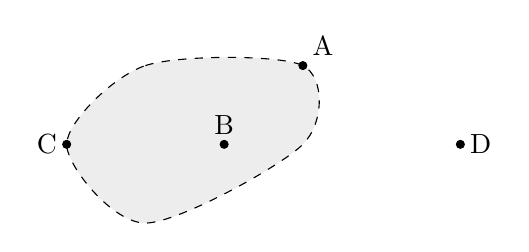
\begin{tikzpicture}
            \draw[fill=lightgray, dashed] plot [smooth cycle] coordinates {(0,0) (1,1) (3,1) (3,0) (1,-1)};
            \draw [fill] (3, 1) circle [radius=0.05];
            \node [above right] at (3,1) {A};
            \draw [fill] (2,0) circle [radius=0.05];
            \node [above] at (2,0) {B};
            \draw [fill] (0,0) circle [radius=0.05];
            \node [left] at (0,0) {C};
            \draw [fill] (5,0) circle [radius=0.05];
            \node [right] at (5, 0) {D};
          \end{tikzpicture}
          \caption{Points $A, B, C$ are limit points of the open set. However, point $D$ is not a limit point. }
          \label{fig:limit_boundary}
        \end{figure}

        \item A point can be at the ``convergence point'' of a sequence. 
        \begin{figure}[H]
          \centering 
          \begin{tikzpicture}
            \draw [fill] (0, 2.2) circle [radius=0.05];
            \draw [fill] (1, 2.4) circle [radius=0.05];
            \draw [fill] (2, 2) circle [radius=0.05];
            \draw [fill] (2.5, 1.8) circle [radius=0.05];
            \draw [fill] (2.6, 1.6) circle [radius=0.05];
            \draw [fill] (2.65, 1.67) circle [radius=0.05];
            \draw [fill] (2.654, 1.64) circle [radius=0.05];
            \draw [fill] (2.6543, 1.63) circle [radius=0.05];
            \node [right] at (2.6543, 1.63) {p};
          \end{tikzpicture}
          \caption{Note that if $S$ is a sequence of points in $\mathbb{R}^{2}$ that converges to $p$ without ever hitting it, we can say that $p \not\in S$ is a limit point of $S$.}
          \label{fig:limit_sequence}
        \end{figure}
      \end{enumerate}
    \end{example}

  \subsection{Basis} 

    So far so good. We want to continue analyzing the properties of a topology, but sometimes working with the entire topology is a bit thorny. There is a tamer representation of a topology, which can also give us the starting point to \textit{construct} topologies. 

    \begin{definition}[Basis]
      If $X$ is a set, a \textbf{basis} on $X$ is a collection $\mathscr{B}$ of subsets of $X$ (called \textbf{basis elements}) such that
      \begin{enumerate}
        \item For each $x \in X$, there is at least one basis element $B \in \mathscr{B}$ containing $x$. That is, the elements of $\mathscr{B}$ covers $X$. 
        \item If $x$ belongs to the intersection of two basis elements $B_1$ and $B_2$, then there is a basis element $B_3$ containing $x$ such that $B_3 \subset (B_1 \cap B_2)$. 
      \end{enumerate}
    \end{definition} 

    The name gives away the clue that a topology may be created from this basis.  

    \begin{theorem}[Basis to Topology]
      Given a basis $\mathscr{B}$ on a set $X$, we can define a topology $\mathscr{T}$, called the \textbf{topology generated by $\mathscr{B}$}, in the following equivalent ways. 
      \begin{enumerate}
        \item $\mathscr{T}$ consists of subsets $U$ of $X$ satisfying the property that for each $x \in U$, there exists a basis element $B \in \mathscr{B}$ such that $x \in B \subset U$. 
        \begin{center}
          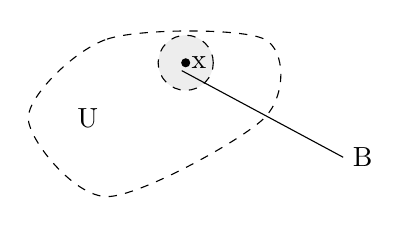
\begin{tikzpicture}
          \draw[dashed] plot [smooth cycle] coordinates {(0,0) (1,1) (3,1) (3,0) (1,-1)};
          \node [right] at (0.5,0) {U};
          \draw[fill=lightgray,dashed] (2,0.7) circle [radius=0.35];
          \draw[fill] (2, 0.7) circle [radius=0.05];
          \node [right] at (1.95,0.7) {x};
          \node [right] at (4,-0.5) {B};
          \draw (1.95,0.6)--(4,-0.5);
          \end{tikzpicture}
        \end{center}

        \item $\mathscr{T}$ consists of all possible unions of elements in $\mathscr{B}$. 
        \begin{equation}
          \mathscr{T} \equiv \Big\{ \bigcup_i b_i \; \Big| \; b_i \in \mathscr{B}\Big\}
        \end{equation}
      \end{enumerate}
    \end{theorem} 
    \begin{proof}
      We prove that the 2 methods generate a topology, and then finally prove that it they are the same topology. 
      \begin{enumerate}
        \item Clearly, $\emptyset$ and $X$ itself are in $\mathscr{T}$. To prove property 2, given a certain indexed family of subsets $\{U_\alpha\}_{\alpha \in I}$ of $\mathscr{T}$, we must show that 
        \begin{equation}
          U = \bigcup_{\alpha \in I} U_\alpha \in \mathscr{T}
        \end{equation}
        Given $x \in U$, there exists at least one index $\alpha$ such that $x \in U_\alpha$. Since $U_\alpha \in \mathscr{T}$ already, there exists a basis element $b \in \mathscr{B}$ such that $x \in b \subset U_\alpha$. But 
        \begin{equation}
          U_\alpha \subseteq U \implies b \subset U
        \end{equation}
        So, by definition, any arbitrary union of $U$ of these subsets is also in $\mathscr{T}$. 

        To prove property 3, we must show that 
        \begin{equation}
          W = \bigcap_{\alpha \in I} U_\alpha \in \mathscr{T}
        \end{equation}
        Given $x \in W$, by definition of a basis element, there exists a $b \in \mathscr{B}$ such that 
        \begin{equation}
          x \in b \subset (U_\beta \cap U_\gamma) \forall \beta, \gamma \in I \implies \text{ there exists } \Tilde{b} \in \mathscr{B} \text{ s.t. } x \in \Tilde{b} \subset \bigcap_{\alpha \in I} U_\alpha
        \end{equation}
        By definition, $W$ is also open. Since this arbitrary set of subsets $\mathscr{T}$ suffices the 3 properties, it is a topology of $X$ by definition. 

        \item $(\rightarrow)$ Given a collection of elements in $\mathscr{B}$, they are also elements of $\mathscr{T}$. Since $\mathscr{T}$ is a topology, their union in also in $\mathscr{T}$. 

        $(\leftarrow)$ Given an open set $U \in \mathscr{T}$, for every point $x \in U$, by definition we can choose a basis element $b \in \mathscr{B}$ such that $x \in b \subset U$. Then, the union of all these basis elements is by definition $b$. 
          
      \end{enumerate}
    \end{proof}

    We have learned how to go from a basis to a topology. The following lemma tells us how to identify a basis within a topology. 

    \begin{theorem}[Topology to Basis]
      Let $X$ be a topological space, and let $\mathcal{C}$ be a collection of subsets of $X$ such that for every open set $U$ and each $x \in U$, there exists an element $c \in \mathcal{C}$ such that
      \begin{equation}
        x \in c \subset U
      \end{equation}
      Then, $\mathcal{C}$ is a basis for the topology of $X$. 
    \end{theorem}
    \begin{proof}
      
    \end{proof}

    \begin{example}[Nested Interval Topology on $(0,1)$]
      In the set $X = (0,1)$, the basis of the \textbf{nested interval topology} is 
      \begin{equation}
        \Big\{ (0, 1-\frac{1}{n}) \; | \; n = 2, 3, ..., \infty \Big\}
      \end{equation}
      In fact, the basis is equivalent to the topology itself! This topology will be denoted $\tau_{NI}$.
    \end{example}

    \begin{example}[Closed Interval Topology on [-1, 1]]
      In the set $X = [-1, 1]$, the basis of the \textbf{closed interval topology} is 
      \begin{equation}
        \big\{ [-1, a) \; | \; a>0 \big\} \bigcup \big\{ (b, 1] \; | \; b<0 \big\} 
      \end{equation}
      This topology will be denoted $\tau_{CI}$
    \end{example}

    \begin{example}[Lower Limit Topology]
      The \textbf{lower limit topology}, denoted $\tau_{LL}$ has basis consisting of half-open intervals in the form $[a, b), a<b$. 
    \end{example}

    \begin{example}[$L_2$-Open Ball Topology]
      The \textbf{open ball topology} on $\mathbb{R}^{n}$ include all open balls of form: 
      \begin{equation}
        B_{r}(p) = \{ x \in \mathbb{R}^{n} \; | \; ||x-p||_2 < r \}
      \end{equation}
      This is the usual topology in $\mathbb{R}^{n}$. It turns out that since all open balls are in $\tau_{\mathbb{R}^{2}}$, we can build any shape using the union/intersections of these open balls, such as an open square. Thus all open subsets in $\mathbb{R}^{n}$ are open sets. 
    \end{example} 

    While it is not surprising that a basis uniquely generates a topology, different bases may generate the same one. The theorem below allows us to work with a ``nicer'' $L_\infty$ metric that only concerns itself with maximums rather than the $L_2$, which uses square roots that may make analysis more tedious. 

    \begin{theorem}[Equal Topologies] 
      The topologies generated by the $L_2$ metric and the $L_\infty$ metric are the same. 
    \end{theorem} 
    \begin{proof}
      Since metrics are nonnegative,\footnote{The ordered field properties of $\mathbb{R}$ can be used to show that for $x, y > 0$, $x < y \iff x^2 < y^2$.} it suffices to show that $\rho(x, y)^2 \leq d(x, y)^2 \leq n \rho (x, y)^2$. For the left-hand side inequality, 
      \begin{align}
        \rho(x, y)^2 & = \big( \max_i |x_i - y_i| \big)^2 && \tag{definition of $L_\infty$ metric}\\
                     & = \max_i | x_i - y_i|^2 && \tag{can move square inside since $|x_i - y_i| > 0$ for all $i$}\\
                     & = \max_i (x_i - y_i)^2 && \tag{absolute value is irrlevant if we are squaring it}\\
                     & \leq \sum_i (x_i - y_i)^2 && \tag{sum contains the max with all nonnegative elements}\\
                     & = d(x, y)^2 && \tag{definition of $L_2$ metric}
      \end{align}
      For the right hand side inequality, we see that 
      \begin{align}
        d(x, y)^2 & = \sum_i (x_i - y_i)^2 && \tag{definition of $L_2$ metric}\\
                  & \leq \sum_i \max_i ( x_i - y_i)^2 && \tag{bound each element by the max of the elements}\\
                  & = n \cdot \max_i (x_i - y_i)^2 && \tag{since it's a sum of constant elements}\\
                  & = n \cdot \big( \max_i (|x_i - y_i|)\big)^2 && \tag{equivalent by previous logic}\\
                  & = n \cdot \rho(x, y)^2 && \tag{definition of $L_\infty$ norm}
      \end{align}
      Assume that $y \in B(x, r)$. Then, we have 
      \begin{equation}
        y \in B(x, r) \iff d(x, y) < r \implies \rho(x, y) < r \iff y \in B_\rho (x, r) 
      \end{equation}
      where the forward implication follows from the transitivity of the metric from 2.b. As the for the second inequality, 
      \begin{align}
        y \in B_\rho (x, \frac{r}{\sqrt{n}}) & \iff \rho(x, y) < \frac{r}{\sqrt{n}}\\ 
                                             & \iff \sqrt{n} \rho(x, y) < r && \tag{$n > 0$}\\
                                             & \implies d(x, y) < r && \tag{transitivity from 2.b}\\
                                             & \iff y \in B(x, r)
      \end{align}
      Now we prove that $\mathscr{T}_2 = \mathscr{T}_\infty$
      \begin{enumerate}
        \item $U$ is $\rho$-open $\implies U$ is open. Let $U$ be $\rho$-open. Then for any $x \in U$, there exists $r > 0$ s.t. $B_\rho (x, r) \subset U$. But since we know that $B(x, r) \subset B_\rho (x, r)$, $r > 0$ also satisfies $B(x, r) \subset U$. Therefore $U$ is open. 

        \item $U$ is open $\implies U$ is $\rho$-open. Let $U$ be open. Then for any $x \in U$, there exists $r > 0$ s.t. $B(x, r) \subset U$. Now choose $\frac{r}{\sqrt{n}} > 0$. We see from 2.c that $B_\rho (x, \frac{r}{\sqrt{n}}) \subset B(x, r)$, and so $B_\rho (x, \frac{r}{\sqrt{n}}) \subset U$ as well.  
      \end{enumerate}
      Therefore the existence of $r$ in one type of openness allows us to guarantee the existence of another $r^\prime$ of another openness. We are done. 
    \end{proof}

  \subsection{Fineness}

    \begin{definition}[Finer, Coarser Topologies]
      Suppose that $\mathscr{T}$ and $\mathscr{T}^\prime$ are two topologies on a given set $X$. If $\mathscr{T} \subset \mathscr{T}^\prime$, we say that $\mathscr{T}^\prime$ is \textbf{finer} than $\mathscr{T}$, or equivalently, we say that $\mathscr{T}$ is \textbf{coarser} than $\mathscr{T}^\prime$. 
    \end{definition}

    We can think of the topology of a set $X$ as a truck full of gravel as the open sets. If the gravel is smashed into smaller, finer pieces, then the amount of stuff that we can make from the finer gravel increases, which corresponds to a bigger topology. The trivial topology is the coarsest topology and the discrete topology is the finest. 

    \begin{lemma}[Fineness w.r.t. Basis]
      Given two topologies $\mathscr{T}$ and $\mathscr{T}^\prime$ with their bases $\mathscr{B}$ and $\mathscr{B}^\prime$, respectively, the following are equivalent. 
      \begin{enumerate}
        \item $\mathscr{T}^\prime$ is finer than $\mathscr{T}$. 
        \item For each $x \in X$ and basis element $b \in \mathscr{B}$ containing $x$, there exists a basis element $b^\prime \in \mathscr{B}^\prime$ such that $x \in b^\prime \subset b$. 
      \end{enumerate}
    \end{lemma}

    \begin{example}
      The set of all open balls $B_r (x)$ with $r, x \in \mathbb{R}$ of $\mathbb{R}^n$ is the basis of the open ball topology. The set of all open boxes in $\mathbb{R}^{n}$ of the form 
      \begin{equation}
        \prod_{i=1}^n [\alpha_i, \beta_i], \; \alpha_i, \beta_i \in \mathbb{R} 
      \end{equation}
      forms a basis of $\tau_{\mathbb{R}^{n}}$. Note that both of these bases generate the same topology. 
    \end{example}

  \subsection{Closed Sets} 

    \begin{definition}[Closed Set]
      The complement of an open set is a \textbf{closed set}. That is, given $x \in \tau_{X}, X \setminus x$ is a closed set. Note that open and closed sets are not mutually exclusive. A set might be open, closed, both, or neither. A set that is both open and closed is called \textbf{clopen}.
    \end{definition}

    \begin{example}[Atoms]
      A point $p$ in $\mathbb{R}^{n}$ is a closed set, since the set $\mathbb{R}^{n} \setminus \{p\}$ can be produced using a infinite union of open balls. 
    \end{example}

    \begin{example}
      Every subset of $X$ with the discrete topology is clopen.
    \end{example}

    \begin{theorem}
      Let $X$ be a topological space. Then, the following conditions hold
      \begin{enumerate}
        \item $\emptyset$ and $X$ are clopen.
        \item Arbitrary intersections of closed sets are closed. 
        \item Finite unions of closed sets are closed. 
      \end{enumerate}
    \end{theorem}

    \begin{definition}
    The \textbf{closure} of set $S \subseteq (X, \tau_{x})$, denoted $\Bar{S}$, is defined as 
    \[ S \bigcup \{\text{all of its limit points}\} \]
    \end{definition}

    \begin{example}
    If $S$ is an open ball, $\Bar{S}$ is the closed ball. 
    \end{example}

    \begin{definition}
    The point $p$ is in the \textbf{interior} of a set $S$ if we can find an open neighborhood $U_p \subseteq S$. It is denoted $S^{o}$. Furthermore, the union of all open sets in $S$ is $S^{o}$. 
    \end{definition}

    \begin{proposition}
    $S$ is open if and only if $S = S^{o}$. $S^{o}$ is always open.
    \end{proposition}

    \begin{theorem}
    The interior $S^{o}$ is the complement of the closure of the complement of S. \[ S^{o} = \big(\overline{S^{c}}\big)^{c}\]
    \end{theorem}

    \begin{definition}
    The \textbf{exterior} of a set $S$ is the complement of the closure, i.e. "strictly outside of $S$ and its boundary."
    \end{definition}

    \begin{definition}
    The \textbf{boundary} of a set $S$, denoted $\partial S$, is the set of points that are neither in the exterior nor the interior, i.e. in the closure, but not the interior of $S$. $p$ is on the \textbf{boundary} of the set $S$ if every neighborhood of $p$ intersects the interior and exterior of $S$.  
    \end{definition}

    \begin{theorem}
    Let $Y$ be a subspace of $X$ with $A$ a subset of $Y$. Let $\bar{A}$ denote the closure of $A$ in $X$. Then, the closure of $A$ in $Y$ equals $\bar{A} \cap Y$. 
    \end{theorem}

    \begin{theorem}
    A subset of a topological space is closed if and only if it contains all of its limit points. That is, 
    \[S = \bar{S}\]
    \end{theorem}

    \begin{definition}
    Let $S \subset (X, \tau_X)$. $S$ is \textbf{dense} in $X$ if every point $p \in X$ is a limit point of $S$. In other words, for any point $p \in X$ and any open neighborhood $U_p$ of $p$, $U_p \cap S$ is nontrivial. Otherwise, $p$ is a point of $S$. 
    \end{definition}

    The following example is a crucial fact for proving further properties of topological spaces. 

    \begin{example}
    $\mathbb{Q}^{n}$ is a dense set of $\mathbb{R}^{n}$ with the open ball topology. If we have the discrete topology of $\mathbb{R}^{2}$, an open neighborhood of a point is the point itself, so no limit points would exist beyond the points in $S$ itself. So $\mathbb{Q}^{n}$ is not dense in $\mathbb{R}^{n}$ with this topology. 
    \end{example}

  \subsection{Continuous Functions}

    \begin{definition}[Continuous Function]
      A function $f$ between 2 topological spaces $(X, \tau_{X})$ and $(Y, \tau_{Y})$ is \textbf{continuous} if the preimage of every open set in $Y$ is an open set in $X$.
      \begin{equation}
        U \in \tau_{Y} \implies f^{-1}(U) \in \tau_{X}
      \end{equation}
      \begin{center}
        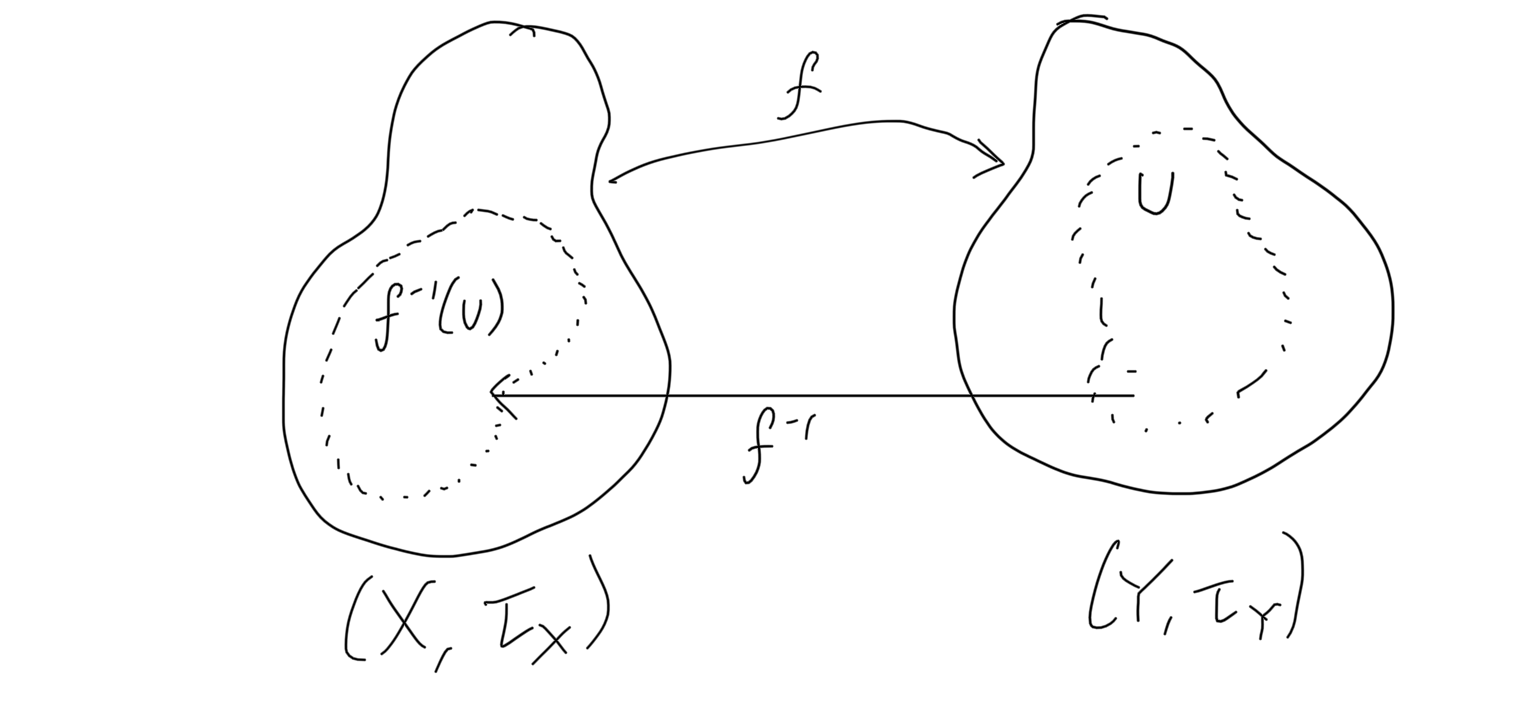
\includegraphics[scale=0.20]{img/Topological_Continuity_of_Functions.PNG}
      \end{center}
      Note that continuity of a function $f$ is not only determined by the function itself, but also by the topologies of $X$ and $Y$. Note also that $f^{-1}$ isn't necessarily a function unless $f$ is injective. Also, this definition of continuity is equivalent to the epislon delta definition of continuity of functions. 
    \end{definition}

    Note that to check if $f$ is continuous, it suffices to check that the preimage of every basis element of the topology of $Y$ under $f$ is open in $X$, since every open set in $Y$ can be constructed as the union of basis elements. More rigorously, an arbitrary open set $V$ of $Y$ can be written as 
    \begin{equation}
      V = \bigcup_{\alpha \in J} b_\alpha
    \end{equation}
    Then, 
    \begin{equation}
      f^{-1} (V) = f^{-1} \Big( \bigcup_{\alpha \in J} b_\alpha \Big) = \bigcup_{\alpha \in J} f^{-1} (b_\alpha)
    \end{equation}

    \begin{theorem}[Sufficient Properties for Continuity]
      Let $X, Y$, be topological spaces and let $f: X \longrightarrow Y$. Then, the following are equivalent. 
      \begin{enumerate}
        \item $f$ is continuous. 
        \item For every subset $A$ of $X$, $f(\bar{A}) \subset \bar{f(A)}$. 
        \item For every closed set $B$ in $Y$, the set $f^{-1} (B)$ is closed in $X$. 
      \end{enumerate}
    \end{theorem}

    \begin{definition}[Homeomorphism]
      A bijective, bicontinuous function 
      \begin{equation}
        f: X \longrightarrow Y
      \end{equation}
      between two topological spaces is called a \textbf{homeomorphism} between $X$ and $Y$. If there exists at least one homeomorphism between $X$ and $Y$, then $X$ is said to be \textbf{homeomorphic} to $Y$. 

      \begin{figure}[H]
        \centering 
        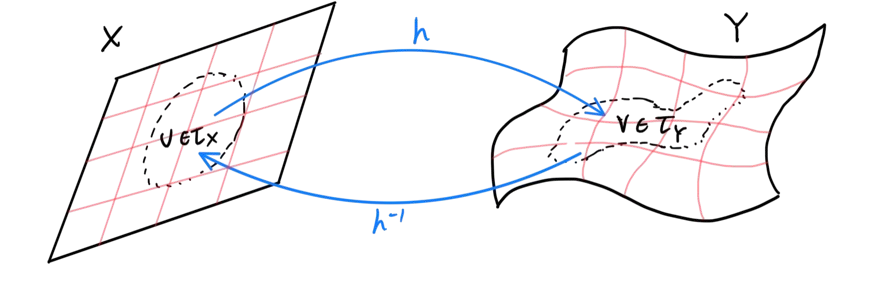
\includegraphics[scale=0.25]{img/Homeomorphism_of_Plane.PNG}
        \caption{The visual below shows a homeomorphism between the plane $X$ and the surface $Y$.}
        \label{fig:homeomorphism_plane}
      \end{figure}
    \end{definition}

    In fact, a homeomorphism $f$ is an equivalence relation between two topological spaces. This partitions the set of all topological spaces into \textbf{homeomorphism classes}. Analogous to how isomorphisms preserve algebraic structures, homeomorphisms preserve topological structure between topological spaces. 

    Additionally, not only does a homeomorphism give a bijective correspondence between points in $X$ and $Y$, but it also determines a bijection between \textbf{the set of all open sets in $X$ and $Y$} (that is, a bijection between their topologies)! This bijection then allows two spaces that are homeormophic to have the same topological properties. 

    \begin{proposition}
      A homeomorphism $f$ between two topological spaces $(X, \tau_{x})$ and $(Y, \tau_{Y})$ preserves all topological properties (e.g. separability, countability, compactness, (path) connectedness) of $X$ onto $Y$ and $Y$ onto $X$. 
    \end{proposition}

    \begin{definition}
      Suppose that $f: X \longrightarrow Y$ an injective continuous map with $X, Y$ topological spaces. Let $Z \equiv \im{f}$. Then, the function
      \begin{equation}
        f^\prime: X \longrightarrow Z \subset Y
      \end{equation}
      obtained by restricting the codomain of $f$ is bijective. If $f^\prime$ happens to be a homeomorphism of $X$ with $Z$, then we say that the map
      \begin{equation}
        f: X \longrightarrow Y
      \end{equation}
      is a \textbf{topological embedding}, or more simply an \textbf{embedding}, of $X$ in $Y$. 
    \end{definition}

    \begin{lemma}[Pasting Lemma, Gluing Lemma]
      Let $X = A \cup B$, where $A, B$ are closed in $X$. Let $f: A \longrightarrow Y$ and $g: B \longrightarrow Y$ be continuous. If 
      \begin{equation}
        f(x) = g(x) \text{ for all } x \in A \cap B
      \end{equation}
      Then $f$ and $g$ can be combined to form a continuous function $h: X \longrightarrow Y$, defined
      \begin{equation}
        h(x) \equiv \begin{cases}
          f(x) & x \in A \setminus B \\
          f(x) \text{ or } g(x) & x \in A \cap B \\
          g(x) & x \in B \setminus A
        \end{cases}
      \end{equation}
      This is shown in the following visual. 
      \begin{center}
          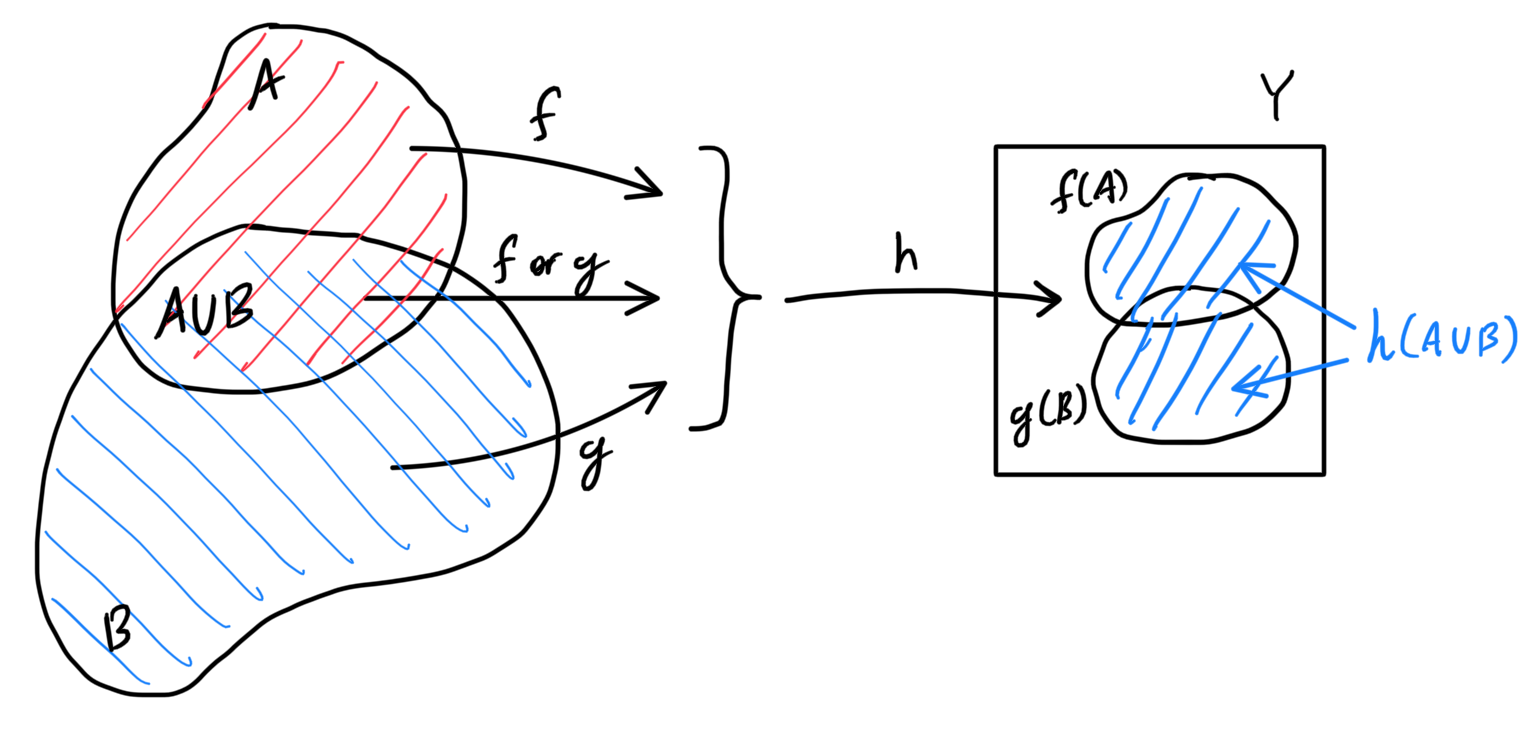
\includegraphics[scale=0.25]{img/Gluing_Lemma.PNG}
      \end{center}
    \end{lemma}

    \begin{theorem}
      Let $f: A \longrightarrow X \times Y$ be given by the equation 
      \begin{equation}
        f(a) \equiv \big( f_1 (a), f_2(a) \big)
      \end{equation}
      Then $f$ is continuous if and only if the function $f_1: A \longrightarrow X$ and $f_2: A \longrightarrow Y$ are continuous. 
    \end{theorem}

    However, there is no useful criterion for the continuity of a mapping 
    \begin{equation}
      f: X \times Y \longrightarrow A
    \end{equation}
    if the domain of $f$ is a product space. One might conjecture that this $f$ is continuous if it is continuous in each variable separately, but this is in fact not true. 

\section{Construction of Topologies} 

  \subsection{Subspace Topologies} 

    \begin{definition}[Subspace Topologies]
    Given topological space $X$ and subspace $Y \subset X$, the topology of $X$ induces the topology of $Y$ in the following way. 
    \[\tau_Y = \{U \cap Y\;|\; U \in \tau_X\}\]
    That is, the open sets of $Y$ are defined to be the intersection of the open sets of $X$ with the space $Y$. This is called the \textbf{subspace topology}. The subspace topology of a line $l$ embedded in $\mathbb{R}^2$ and that of a surface $\mathcal{L}$ embedded in $\mathbb{R}^3$ is shown. 
    \begin{center}
        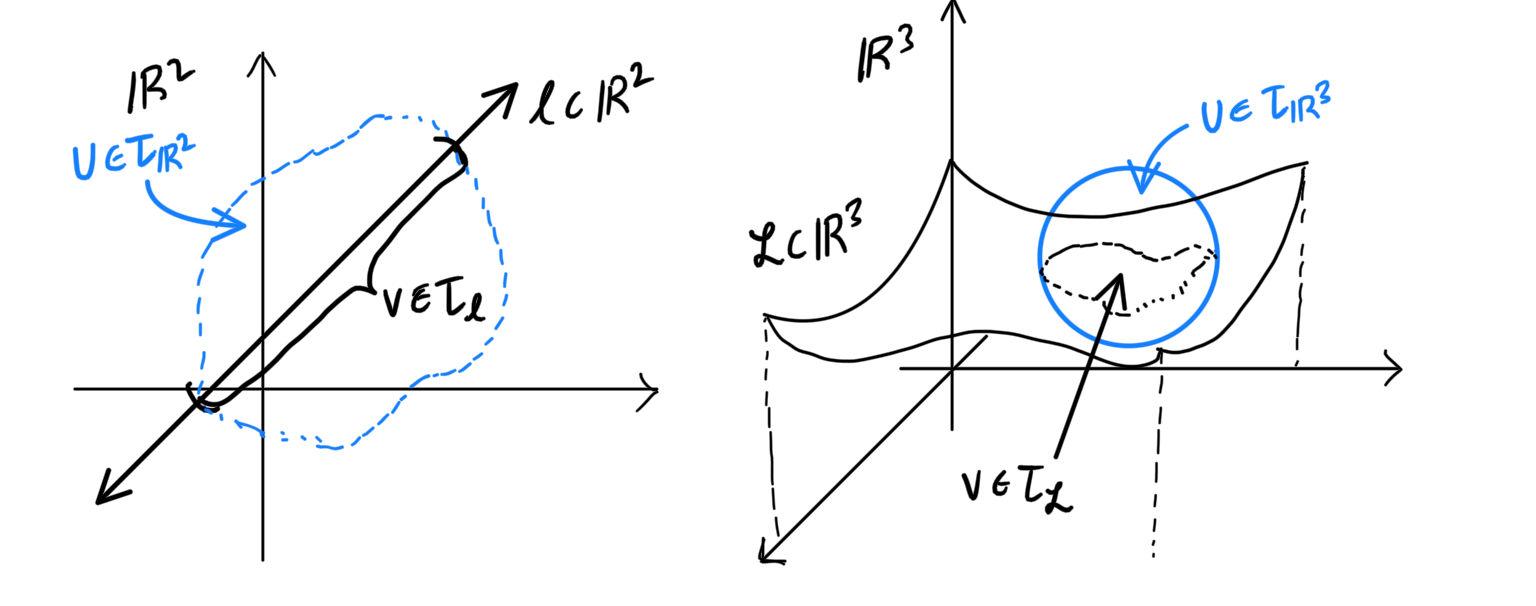
\includegraphics[scale=0.25]{img/Subspace_Topology.PNG}
    \end{center}
    \end{definition}

  \subsection{Box and Product Topologies} 

    There are multiple ways to define the box and product topologies, but their construction with basis elements is most simple. 

    \begin{definition}
    Let $\{X_\alpha\}_{\alpha \in I}$ be an indexed (finite or countably infinite) family of topological spaces and let us take the product of these spaces
    \[\prod_{\alpha \in I} X_\alpha\]
    We could endow the \textbf{box topology} of all open sets in the form
    \[\prod_{\alpha \in I} U_\alpha\]
    where $U_\alpha$ is open in $X_\alpha$ for each $\alpha \in I$. It is clear that a basis element $B$ of the box topology is of form
    \[B = \prod_{\alpha \in I} B_\alpha\]
    where $B_\alpha$ is a basis element of the topology of each component space $X_\alpha$. 
    \end{definition}

    We can visualize the elements of the box topology with the product space $\mathbb{R}^2 = \mathbb{R} \times \mathbb{R}$, where each $\mathbb{R}$ has an open ball topology. From the visual below, we can see why this is called the "box" topology. Furthermore, all basis elements of this space are arbitrary open rectangles in $\mathbb{R}^2$. 
    \begin{center}
    \begin{tikzpicture}
        \draw[<->] (-1,0)--(6,0);
        \draw[<->] (0,-1)--(0,4);
        \draw[dashed] (1,1)--(1,3)--(4,3)--(4,1)--(1,1);
        \node[below] at (6,0) {$\mathbb{R}$};
        \node[left] at (0,4) {$\mathbb{R}$};
        \node[below] at (1,-0.3) {$a$};
        \node[below] at (4,-0.3) {$b$};
        \node[left] at (-0.3,1) {$c$};
        \node[left] at (-0.3,3) {$d$};
        \node[rotate=90] at (0,1) {$($};
        \node[rotate=-90] at (0,3) {$($};
        \node at (1,0) {$($};
        \node at (4,0) {$)$};
    \end{tikzpicture}
    \end{center}

    It is easy to prove that the box topology indeed satisfies the 3 properties of topologies in general. While this topology may seem quite "intuitive" for the first learner, the box topology, however, has serious limitations when extending to infinite Cartesian products of spaces. Let 
    \[\pi_\beta: \prod_{\alpha \in I} X_\alpha \longrightarrow X_\beta, \; \pi_\beta \big( (x_\alpha)_{\alpha \in I}\big) \equiv x_\beta\] 
    be the projection mapping of an element in the product space to the $\beta$th space. 

    \begin{definition}
    Let $\{X_\alpha\}_{\alpha \in I}$ be an indexed family of topological spaces with their product space defined as above. Given an open set $U_\beta \subset X_\beta$, let us define $\mathscr{S} (U_\beta) \subset \prod X_\alpha$ as 
    \begin{align*}
        \mathscr{S}(U_\beta) \equiv X_1 \times X_2 \times ... \times X_{\beta -1} \times U_\beta \times X_{\beta+1} \times ... 
    \end{align*}
    Visually, we can interpret each $\mathscr{S} (U_\beta)$ as a "strip" in the total product space. For example in $\mathbb{R}^2$, there are two "strips" $(e, f) \times \mathbb{R}$ and $\mathbb{R} \times (g, h)$ that intersect. 
    \begin{center}
    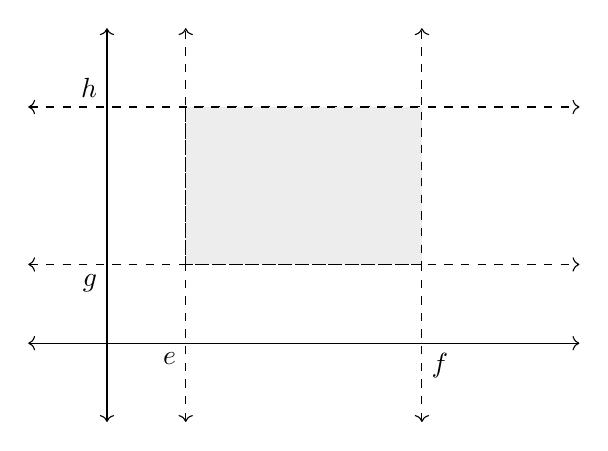
\begin{tikzpicture}
        \draw[<->] (-1,0)--(6,0);
        \draw[<->] (0,-1)--(0,4);
        \draw[<->, dashed] (-1,1)--(6,1);
        \draw[<->, dashed] (-1,3)--(6,3);
        \draw[<->, dashed] (1,-1)--(1,4);
        \draw[<->, dashed] (4,-1)--(4,4);
        \node [below left] at (1,0) {$e$};
        \node [below right] at (4,0) {$f$};
        \node [above left] at (0,3) {$h$};
        \node [below left] at (0,1) {$g$};
        \draw[dashed, fill=lightgray] (1,1) rectangle (4,3);
    \end{tikzpicture}
    \end{center}
    The topology generated by this basis is called the \textbf{product topology}. Note that by the properties of topologies, we can create open sets by taking unions and finite intersections of these basis elements. This means that every open set in the product topology has form
    \[\prod_{\alpha \in I} U_\alpha\]
    where $U_\alpha$ is an open subset of $X_\alpha$ for finitely many $\alpha$'s and $U_\alpha = X_\alpha$ for the rest. 
    \end{definition}

    We can deduce some conclusions comparing these topologies. First, the product and box topologies are precisely the same if we work in finite Cartesian products of spaces, since any element of the box topology (left hand side) can be expressed as a finite intersection of some open sets (in the right hand side). That is, if $\text{card}\,I < \infty$, then 
    \[\prod_{\alpha \in I} U_i = \bigcap_{\alpha \in I} \big\{ \prod_{\gamma \in I} W_\gamma \; | \; W_\gamma = U_\gamma \text{ if } \gamma = \alpha, \, W_\gamma = X_\gamma \text{ if } \gamma \neq \alpha\big\}\]
    Secondly, we can see that the box topology is finer than the product topology (strictly finer if working in infinite product spaces). 

    \begin{example}
    The set $(0,1)^\mathbb{N} \subset \mathbb{R}^\mathbb{N}$ is clearly open in the box topology, but it is considered "too tight" to be in the product topology. However, 
    \[(0,1) \times \mathbb{R} \times \mathbb{R} \times ... \]
    is open in the product topology since only one (a finite amount) of the factors is not the whole space. 
    \end{example}

    The main difference between the construction of open sets in the box topology vs the product topology is that the box topology merely describes open sets as direct products of open sets from each coordinate space. That is,
    \[U_\alpha \text{ open in } X_\alpha \implies \prod_{\alpha \in I} U_\alpha \text{ open in } \prod_{\alpha \in I} X_\alpha\]
    On the other hand, the construction of the product topology is completely dependent on the construction of the projection mappings 
    \[ \pi_\beta: \prod_{\alpha \in I} X_\alpha \longrightarrow X_\beta\]
    to be continuous (and nothing more) so that (by definition) the preimages of open sets in $X_\beta$ under $\pi_\beta$ are open sets in $\prod X_\alpha$. Therefore, the construction of the continuous $\pi_\beta$'s canonically constructs a basis of open sets in $\prod X_\alpha$. Taking the union and finite intersection of these open sets gives us the product topology. 

    \begin{theorem}
    If each space $X_\alpha$ is a Hausdorff space, then 
    \[\prod_{\alpha} X_\alpha\]
    is also Hausdorff in both the box and product topologies. 
    \end{theorem}

    The following theorem reveals why the product topology is superior than the box topology in product spaces. 

    \begin{theorem}
    Given the function 
    \[f: A \longrightarrow \prod_{\alpha \in I} X_\alpha, \; f(a) \equiv \big( f_\alpha (a) \big)_{\alpha \in I}\]
    with its component functions $f_\alpha: A \longrightarrow X_\alpha$. Let $\prod X_\alpha$ have the product topology. Then the function $f$ is continuous if and only if each function $f_\alpha$ is continuous. 
    \end{theorem}
    \begin{proof}
    Let $\pi_\beta$ be the projection of this product onto the $\beta$th component space. By construction $\pi_\beta$ is continuous $\implies \pi_\beta^{-1} (U_\beta)$ is a basis element of the product topology of $\prod X_\alpha$. \\
    $(\rightarrow)$ $f$ is continuous, so $f_\beta \equiv \pi_\beta \circ f$, as the composition of continuous functions, is also continuous. \\
    $(\leftarrow)$ Assume that each $f_\beta$ is continuous. Let there be an open set $U_\beta \subset X_\beta$. Then, the canonical open set $\pi_\beta^{-1}$ in the product space $\prod X_\alpha$ is also open. Now, the preimage of $\pi_\beta^{-1} (U_\beta)$ under $f$ is \begin{align*}
        f^{-1} \big( \pi_\beta^{-1} (U_\beta)\big) & = (f^{-1} \circ \pi_\beta^{-1})(U_\beta) \\
        & = (\pi_\beta \circ f)^{-1} (U_\beta) \\
        & = f_\beta^{-1} (U_\beta)
    \end{align*}
    Since $f_\beta$ is already assumed to be continuous, $f_\beta^{-1} (U_\beta)$ is open in $A$. 
    \end{proof}

    This theorem also works for the box topology only if we are working with finite product spaces. But in general, this theorem fails for the box topology. Consider the following example. 

    \begin{example}
    Let $\mathbb{R}^\omega$ be the countably infinite product of $\mathbb{R}$'s. Let us define the function 
    \[f: \mathbb{R} \longrightarrow \mathbb{R}^\omega\]
    with coordinate function defined $f_n (t) \equiv t$ for all $n \in \mathbb{N}$. Clearly, each $f_n$ is continuous. Given the box topology, we consider one basis element of $\mathbb{R}^\omega$
    \[B = \prod_{i=1}^\infty (-\frac{1}{i}, \frac{1}{i})\]
    Assume that $f$ is continuous, that is $f^{-1}(B)$ is open in $\mathbb{R}$. Then, it would contain some finite interval $(-\delta, \delta)$ about $0$, meaning that $f\big( (-\delta, \delta)\big) \subset B$. This implies that for each $n \in \mathbb{N}$, 
    \[f_n \big( (-\delta, \delta) \big) = (-\delta, \delta) \subset \Big( -\frac{1}{n}, \frac{1}{n} \Big)\]
    which contradicts the fact that $B$ is open, since the interval $(-1/n, 1/n)$ converges onto a point $0$. 
    \end{example}

  \subsection{Order, Dictionary Topologies} 

    \begin{definition}[Order Topology]
      Let $X$ be a set with a simple order relation. Let $\mathscr{B}$ be the collection of all sets of the following types. 
      \begin{enumerate}
        \item All open intervals $(a, b) \subset X$
        \item All half-open intervals $[a_0, b)$, where $a_0$ is the minimum element of $X$
        \item All half-open intervals $(a, b_0]$, where $b_0$ is the maximum element of $X$. 
      \end{enumerate}
      This set $\mathscr{B}$ is a basis for the \textbf{order topology} of $X$. If $X$ has no minimum or maximum, then there are no sets of type of 2 or 3, respectively. 
    \end{definition}

    \begin{example}
      The standard topology on $\mathbb{R}$ is precisely the order topology derived from the usual order on $\mathbb{R}$. 
    \end{example}

    \begin{example}
      Given $\mathbb{R} \times \mathbb{R}$ with the dictionary order, then $\mathbb{R} \times \mathbb{R}$ has neither a largest nor smallest element. Therefore, the order topology on $\mathbb{R} \times \mathbb{R}$ consists of all "intervals" of form
      \[\big((a, b), (c, d) \big) \equiv  \{(x, y) \in \mathbb{R}^2 \; | \; (a, b) < (x, y) < (c, d)\}\]
      A visual diagram is shown below. This means that open rays and lines are also a part of the topology of $\mathbb{R} \times \mathbb{R}$. 

      \begin{center}
      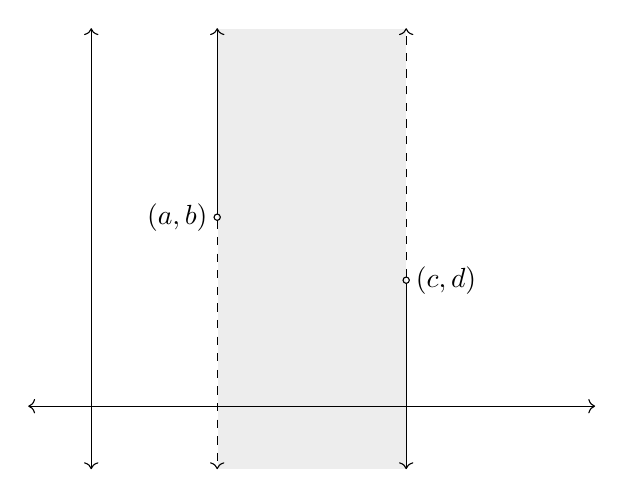
\begin{tikzpicture}[scale=0.8]
          \draw[white, fill=lightgray] (2,-1) rectangle (5,6);
          \draw[<->] (-1,0)--(8,0);
          \draw[<->] (0,-1)--(0,6);
          \draw[->] (2,3.05)--(2,6);
          \draw[->] (5,1.95)--(5,-1);
          \draw (2,3) circle [radius=0.05];
          \draw (5,2) circle [radius=0.05];
          \draw[dashed, ->] (2,2.95)--(2,-1);
          \draw[dashed,->] (5,2.05)--(5,6);
          \node[left] at (2,3) {$(a, b)$};
          \node[right] at (5,2) {$(c,d)$};
      \end{tikzpicture}
      \end{center}
    \end{example}

    \begin{example}
      The set of positive integers $\mathbb{Z}_+$ form an ordered set with a smallest element. The order topology for $\mathbb{Z}_+$ is precisely the discrete topology since every one-point set is an open set. 
      \[\{n\} = (n-1, n+1)\]
    \end{example}

    \begin{example}
      The dictionary order topology on $\{1, 2\} \times \mathbb{Z}_+$ results in every one point set being open, except for the point $(2, 1)$. Since every neighborhood of $(2,1)$ must contain some point of form $(1, n)$ for arbitrarily large $n$, $\{(2,1)\}$ is not open. 
    \end{example}

    \begin{definition}
      If $X$ is an ordered set a $a \in X$, then there are 4 subsets of $X$ called rays determined by $a$. 
      \begin{enumerate}
        \item $(a, +\infty)$ 
        \item $(-\infty, a)$
        \item $[a, +\infty)$
        \item $(-\infty, a]$
      \end{enumerate}
      The first two sets are called \textbf{open rays}, and the latter two sets are called \textbf{closed rays}. 
    \end{definition}

  \subsection{Quotient Topologies}

    \begin{definition}
    Let $X$ and $Y$ be topological spaces, and let $p: X \longrightarrow Y$ be a surjective map. The map $p$ is said to be a \textbf{quotient map} if
    \[U \text{ is open in } Y \iff p^{-1}(U) \text{ is open in } X\]
    \end{definition}

    Note that the conditions for being a quotient map is stronger then regular continuity. It is sometimes called \textbf{strong continuity}. An equivalent condition for $p$ to be a quotient map is to require that given $A \subset Y$, 
    \[A \text{ closed in } Y \iff p^{-1}(A) \text{ closed in } X\]
    This equivalence follows from the fact that
    \[f^{-1}(Y \setminus B) = X \setminus f^{-1}(B)\]

    \begin{definition}
    A subset $C \subset X$ is \textbf{saturated} with respect to the surjective map $p: X \longrightarrow Y$ if for every $p^{-1} (A)$ (where $A \subset Y$) that intersects $C$, $p^{-1}(A)$ is completely contained within $C$. That is, 
    \[p^{-1} \big( p(C) \big) = C\]
    \end{definition}

    In the visual below, we can see that $C_1$ and $C_2$ alone are not saturated, but $C_1 \cup C_2$ is saturated. Visually, for a given set $C \subset X$ to be saturated, there cannot be any points $q \not\in C$ such that $q \in p(C)$. 

    \begin{center}
    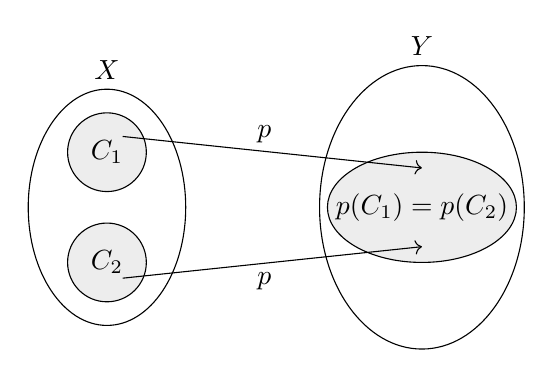
\begin{tikzpicture}
        \draw (0,0) ellipse (1 and 1.5);
        \draw[fill=lightgray] (0, 0.7) circle (0.5);
        \draw[fill=lightgray] (0, -0.7) circle (0.5);
        \node[above] at (0,1.5) {$X$};
        \draw (4,0) ellipse (1.3 and 1.8);
        \node[above] at (4,1.8) {$Y$};
        \draw[fill=lightgray] (4,0) ellipse (1.2 and 0.7);
        \node at (0, 0.7) {$C_1$};
        \node at (0,-0.7) {$C_2$};
        \node at (4,0) {$p(C_1) = p(C_2)$};
        \draw[->] (0.2,0.9)--(4,0.5);
        \draw[->] (0.2,-0.9)--(4,-0.5);
        \node[above] at (2, 0.7) {$p$};
        \node[below] at (2, -0.7) {$p$};
    \end{tikzpicture}
    \end{center}
    We now introduce an alternative, equivalent definition of quotient maps. 

    \begin{definition}
    $p: X \longrightarrow Y$ is a quotient map if and only if $p$ is continuous and $p$ maps saturated open sets of $X$ to open sets of $Y$ (or saturated closed sets of $X$ to closed sets of $Y$). 
    \end{definition}

    \begin{proposition}
    If $p: X \longrightarrow Y$ is a surjective, continuous map that is either open or closed (that is, maps open sets to open sets or closed sets to closed sets), then $p$ is a quotient map. 

    Note however, that the converse is not true; there exists quotient maps that are neither open nor closed. 
    \end{proposition}

    \begin{definition}
    If $X$ is a space and $A$ is a set and if $p: X \longrightarrow A$ is a surjective map, then there exists exactly one topology $\mathscr{T}$ on $A$ relative to which $p$ is a quotient map. $\mathscr{T}$ is called the \textbf{quotient topology} induced by $p$. 
    \end{definition}

    To construct the quotient topology for the surjective map $p$, we must make $p$ continuous. Therfore, the topology $\mathscr{T}$ on $A$ is defined by letting it consist of all subsets $U$ of $A$ such that $p^{-1}(U)$ is open in $X$. This is indeed a topology since
    \begin{enumerate}
        \item $p^{-1} (\emptyset) = \emptyset$ and $p^{-1}(A) = X$
        \item $p^{-1} \Big( \bigcup_{\alpha \in J} U_\alpha \Big) = \bigcup_{\alpha \in J} p^{-1} (U_\alpha)$
        \item $p^{-1} \Big( \bigcap_{i=1}^n U_i \Big) = \bigcap_{i=1}^n p^{-1} (U_i)$
    \end{enumerate}

    We can also construct the quotient topology as the final topology. 

    \begin{definition}
    Given a mapping 
    \[f: (X, \tau_X) \longrightarrow (Y, \tau_Y)\]
    where $\tau_X$ is well-defind and $\tau_Y$ is not, the finest possible topology available on $Y$ that makes $f$ continuous is called the \textbf{final topology of $Y$}. 
    \end{definition}

    Note that we say the "finest possible topology" when defining the final topology. It is because if $\tau_Y$ is too fine (e.g. if $\tau_Y = 2^Y$), then the open sets of $\tau_Y$ would be too fine and therefore would have a preimage that may not be open in $X$. 

    \begin{example}
    Let $p: (\mathbb{R}, \tau_\mathbb{R}) \longrightarrow \mathbb{R} / 2 \pi \mathbb{R}$. Then, the final topology of $\mathbb{R} / 2 \pi \mathbb{R}$ would be simply defined 
    \[\tau_{\mathbb{R} / 2 \pi \mathbb{R}} \equiv \{U \subset \mathbb{R} / 2\pi \mathbb{R} \; | \; U = p(O), O \in \tau_\mathbb{R}\}\]
    That is, the quotient topology is merely the set of all images of open sets in $\mathbb{R}$ under $f$. However, if $\mathbb{R} / 2 \pi \mathbb{R}$ has the discrete topology $2^X$, then a single equivalence class, say $[0]$, will get mapped to the collection of points $\{2 \pi k \; | \; k \in \mathbb{Z}\}$, which is clearly not open in $\mathbb{R}$. Note that the final topology (or the quotient topology) is endowed onto the codomain in order to make $f$ continuous (or a quotient mapping). 
    \end{example}

    \begin{proposition}
    Given a relation $\sim$ on a topological space $(X, \tau_X)$, the quotient topology of the quotient space $X / \sim$, is precisely the final topology on the quotient set with respect to the quotient map $p: X \longrightarrow X / \sim$. That is, 
    \[\tau_{X / \sim} \equiv \big\{U \subseteq X / \sim \; | \; \{x \in X \; | \; p(x) \in U\} \in \tau_X \big\}\]
    which is the topology whose open sets are the subsets of $X / \sim$ that have an open preimage under the surjective map $p: x \mapsto [x]$. 
    \end{proposition}

    \begin{example}
    Let $X \equiv [0,1] \cap [2,3] \subset \mathbb{R}$ and $Y y \equiv [0,2] \subset \mathbb{R}$. Then, we define $p: X \longrightarrow Y$ as 
    \[p(x) \equiv \begin{cases}
          x & x \in [0,1] \\
          x-1 & x \in [2,3]
    \end{cases}\]
    $p$ is continuous (under subspace topology of $X \subset \mathbb{R}$), surjective, and closed, meaning that it is a quotient map. However, it is not open, since the image of the open set $[0,1]$ of $X$ is $[0,1]$, which is not open in $Y$. 
    \end{example}

    \begin{example}
    Let $p: \mathbb{R} \longrightarrow \{a, b, c\}$ be defined as 
    \[p(x) \equiv \begin{cases}
          a & x > 0 \\
          b & x < 0 \\
          c & x = 0
    \end{cases}\]
    Then, the quotient topology of $\{a, b, c\}$ consists of 
    \[\emptyset, \{a\}, \{b\}, \{a, b\}, \{a, b, c\}\]
    \end{example}

    \begin{definition}
    Let $X$ be a topological space, and let $\Tilde{X}$ be a partition of $X$ into disjoint subsets whose union is $X$. Let $p: X \longrightarrow \Tilde{X}$ be the surjective map mapping every point $x \in X$ to the subset that it is in. In the quotient topology induced by $p$, $\Tilde{X}$ is called the quotient space of $X$. 
    \end{definition}

    To construct a quotient space, we can equivalently define a relation on $X$. That is, a subset $U$ of $\Tilde{X}$ is a collection of equivalence classes, and the set $p^{-1}(U)$ is the union of equivalence classes belonging to $U$. Therefore, the typical open set of $\Tilde{X}$ is a collection of equivalence classes whose union is an open set in $X$. 

    \begin{example}[Construction of a Torus]
    Let $X \equiv [0,1] \times [0,1] \subset \mathbb{R}^2$. We define an equivalence relation $Y$ consisting of the equivalence classes
    \begin{align*}
        &\big\{\{(x, y)\} \; | \; 0<x, y<1\big\} \cup \big\{ \{(x, 0), (x,1)\} \; | \; 0<x<1 \big\} \cup \\
        &\big\{ \{(0,y), (1,y)\} \; | \; 0<y<1 \big\} \cup \big\{ \{(0,0), (0,1), (1,0), (1,1)\} \big\}
    \end{align*}
    Then, the quotient topology of this quotient space consists of open sets of form
    \begin{center}
    \begin{tikzpicture}
        \draw (0,0) rectangle (2,2);
        \draw (3,0) rectangle (5,2);
        \draw (6,0) rectangle (8,2);
        \draw (9,0) rectangle (11,2);
        \draw[dashed] (1, 1.5) circle [radius=0.4];
        \draw[fill] (1, 1.5) circle [radius=0.03];
        \draw[dashed] (3.9,0) arc (0:180: 0.4);
        \draw[dashed] (3.9,2) arc (0:-180:0.4);
        \draw[dashed] (6,1.1) arc (-90:90:0.4);
        \draw[dashed] (8,1.9) arc (90:270:0.4);
        \draw[fill] (3.5,0) circle [radius=0.03];
        \draw[fill] (3.5,2) circle [radius=0.03];
        \draw[fill] (6,1.5) circle [radius=0.03];
        \draw[fill] (8,1.5) circle [radius=0.03];
        \draw[fill] (9,0) circle [radius=0.03];
        \draw[fill] (11,0) circle [radius=0.03];
        \draw[fill] (9,2) circle [radius=0.03];
        \draw[fill] (11,2) circle [radius=0.03];
        \draw[dashed] (9.4,0) arc (0:90:0.4);
        \draw[dashed] (9.4,2) arc (0:-90:0.4);
        \draw[dashed] (11,0.4) arc (90:180:0.4);
        \draw[dashed] (10.6,2) arc (180:270:0.4);
    \end{tikzpicture}
    \end{center}
    This quotient space $X / Y$ is homeomorphic to the torus $S^1 \times S^1$, denoted
    \[\frac{X}{Y} \cong S^1 \times S^1\]
    We can visualize the construction of the equivalence relation $Y$ as a "gluing" of the rectangle $X$ by its edges and corners. 

    We can check that this mapping is indeed a quotient map. First, it is clearly surjective. By realizing that individual points on the edge of $[0,1]^2$ are open sets themselves (by the subspace topology), we can prove that this map is indeed open and continuous. 
    \end{example}

    \begin{example}[Construction of the 2-Sphere]
    Let $X$ be the closed unit ball 
    \[X \equiv \{(x, y) \in \mathbb{R}^2 \; | \; x^2 + y^2 \leq 1\}\]
    and define the equialence classes $R$ as 
    \[R \equiv \big\{ \{(x, y)\} \; | \; x^2 + y^2 <1 \big\} \cup \{S^1\}\]
    which will consist of open sets of one of the two forms
    \begin{center}
    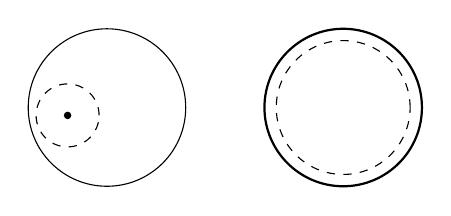
\begin{tikzpicture}
        \draw (1,1) circle [radius=1];
        \draw[thick] (4,1) circle [radius=1];
        \draw[dashed] (0.5,0.9) circle [radius=0.4];
        \draw[fill] (0.5,0.9) circle [radius=0.04];
        \draw[dashed] (4,1) circle [radius=0.85];
    \end{tikzpicture}
    \end{center}
    Then, this quotient space $X / R$ is homeomorphic to the 2-sphere
    \[S^2 \equiv \{(x, y, z) \in \mathbb{R}^3 \; | \; x^2 + y^2 + z^2 = 1\}\]
    Visually, we can imagine the disk being glued together by its sides to continuously form the 2-sphere. 
    \end{example}

    \begin{example}[Construction of the 1-Sphere]
    We will show that
    \[\frac{\mathbb{R}}{\mathbb{Z}} \cong S^1\]
    Let us construct the set $(\mathbb{R}, \tau_{\mathbb{R}})$ with paramater $t$. We define maps
    \begin{align*}
    p: \mathbb{R} \longrightarrow \mathbb{R} / \mathbb{Z}, \;\; p(t) \equiv t \; (\text{mod } 1) \\
    q: \mathbb[R] \longrightarrow S^1 \subset \mathbb{C}, \;\; g(t) \equiv e^{2 \pi i t} 
    \end{align*}
    We claim that $p$ and $q$ are both quotient mappings. Clearly, $p$ is a quotient mapping. As for $q$, it it easy to see that it is surjective (but not injective) and continuous ($\tau_{S^1}$ has the basis of open intervals on $S^1$). It is also easy to notice that given an open interval $U \subset S^1$, $q^{-1}(U)$ will be the union of open intervals equally spaced in $\mathbb{R}$. Additionally, given any open interval in $\mathbb{R}$, it maps to an open interval in $S^1$ (note that $S^1$ itself is also open). These three conditions imply that $q$ is a quotient map. We now define maps 
    \[ q \circ p^{-1}: \mathbb{R} / \mathbb{Z} \longrightarrow S^1 \]
    \[ p \circ q^{-1}: S^1 \longrightarrow \mathbb{R} / \mathbb{Z} \]
    and claim that these maps are homeomorphisms. We can clearly see that the mapping from an open set in $\mathbb{R} / \mathbb{Z}$ to the union of spaced open intervals in $\mathbb{R}$ is an injection, and the mapping from this union of open intervals to the union of open intervals in $S^1$ is a surjection. The composition of these two mappings clearly defines a bijection. Therefore, $q \circ p^{-1}$ is proven to be a bicontinuous bijective mapping between open sets $U \subset \mathbb{R} / \mathbb{Z}$ and $V \subset S^1 \implies$ $q \circ p^{-1}$ is a homeomorphism. 

    This result clearly makes sense since 
    \[\frac{\mathbb{R}}{\mathbb{Z}} \cong \frac{[0,1]}{\sim}\]
    where the relation $\sim$ maps every point $x \in (0,1)$ to its own equivalence class and the points $0, 1$ to one equivalence class $\{0\}$. Therefore, it is informally said that the quotient space of the real line is a circle. 

    One may attempt to construct a simpler set by replacing $S^1$ with the half-open interval $[0,1)$. However, while $[0,1)$ is bijective to $\mathbb{R} / \mathbb{Z}$,
    \[\frac{\mathbb{R}}{\mathbb{Z}} \not\cong [0,1)\]
    That is, the two sets are not homeomorphic because the topologies of $[0,1)$ and $\mathbb{R} / \mathbb{Z}$ are not compatible. For instance, when we attempt to map the open set 
    \[ \bigg\{ [x] \in \mathbb{R} / \mathbb{Z} \; | \; 0 \leq x \leq \frac{1}{4} \vee x > \frac{1}{2} \bigg\} \in \tau_{\mathbb{R} / \mathbb{Z}} \]
    to $\tau_{[0,1)}$, it does not return an open set. 


    Furthermore, this means that
    \[S^1 \times S^1 \cong \frac{[0,1]^2}{\sim^\prime} \cong \bigg( \frac{\mathbb{R}}{\mathbb{Z}} \bigg)^2\]
    where $\sim^\prime$ is the quotient mapping defined in the previous construction of the torus. 
    \end{example}

    \begin{example}[Construction of the Cylinder]
    Let us define the cylinder as 
    \[C \equiv \{(x, y, z) \in \mathbb{R}^3 \; | \; x^2 + y^2 = 1, z \in [0,1]\} \]
    Then, we can see that
    \[C \cong \frac{[0,1]^2}{\sim}\]
    where $\sim$ is the equivalence relation defined by the quotient mapping 
    \[p\big((x, y)\big) \equiv \begin{cases}
          \{(x, y)\} & x \neq 0, x \neq 1 \\
          \{(0,y), (1, y)\} & x = 0 \text{ or } x = 1
    \end{cases}\]
    \end{example}

    Subspaces do not behave well under quotient maps. That is, if $p: X \longrightarrow Y$ is a quotient map and $A$ is a subspace of $X$, then the map $p^\prime: A \longrightarrow p(A)$ obtained by restricting both the domain and codomain of $P$ need not be a quotient map. Additionally, quotient maps are clearly not homeomorphisms, so topological properties are not preserved. 

    However, composites of maps do behave nicely. 

    \begin{proposition}
    The composition of two quotient maps is a quotient map. 
    \end{proposition}
    \begin{proof}
    Indeed, the composition of surjective, continuous, and open maps is surjective, continuous, and open. 
    \end{proof}

    However, the product of two quotient maps is not necessarily a quotient map. That is, given $p: A \longrightarrow B$ and $q: C \longrightarrow D$ are quotient maps, the map 
    \[p \times q: A \times C \longrightarrow B \times D, \; (p \times q) (a \times c) \equiv p(a) \times q(c)\]
    is not necessarily a quotient map. 

    \begin{example}
    Given $(\mathbb{R}, \tau_{\mathbb{R}})$, let us define the relation $\sim$ determined by the quotient mapping
    \[p(x) \equiv \begin{cases}
          \{x\} & x \not\in \mathbb{Z} \\
          \mathbb{Z} & x \in \mathbb{Z}
    \end{cases}\]
    In words, this quotient map maps every integer to the equivalence class $[0]$ and maps every other point to its own class. It turns out that every interval $[j, j+1] \subset \mathbb{R}, \; j \in \mathbb{Z}$ will get mapped as a closed loop in $\mathbb{R} / \sim$ beginning and ending with $[0]$, since $j, j+1 \mapsto [0]$. So geometrically, $\mathbb{R} / \sim$ consists of an infinite number of nonintersecting closed loops starting and ending with $[0]$. 
    \begin{center}
    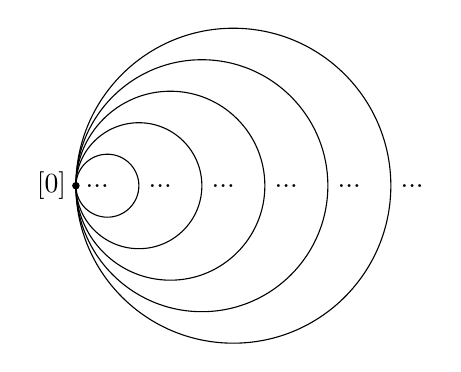
\begin{tikzpicture}[scale=0.4]
        \draw (5,0) circle (5);
        \node[left] at (0,0) {$[0]$};
        \draw[fill] (0,0) circle (0.1);
        \draw (4,0) circle (4);
        \draw (3,0) circle (3);
        \draw (2,0) circle (2);
        \draw (1,0) circle (1);
        \node[right] at (0,0) {...};
        \node[right] at (2,0) {...};
        \node[right] at (4,0) {...};
        \node[right] at (6,0) {...};
        \node[right] at (8,0) {...};
        \node[right] at (10,0) {...};
    \end{tikzpicture}
    \end{center}

    This wacky mapping is an example of a quotient mapping that does not preserve topological structure. While it will not be proven here, it is known that $(\mathbb{R}, \tau_{\mathbb{R}})$ is 1st and 2nd countable, but $\mathbb{R} / \sim$ under this relation is not even 1st countable. 
    \end{example}

    We now introduce theorems of continuous maps from quotient spaces inducing other continuous maps. 

    \begin{theorem}
    Let $p: (X, \tau_X) \longrightarrow (Y, \tau_Y)$ be a quotient map. Let $(Z, \tau_Z)$ be a topological space and let there exist a function $f: Y \longrightarrow Z$. $f$ is continuous if and only if $f \circ p$ is continuous. 
    \[\begin{tikzcd}
        X \arrow{d}{p} \arrow{rd}{f \circ p}\\
        Y \arrow{r}{f} & Z
    \end{tikzcd}\]
    \end{theorem}
    \begin{proof}
    ($\rightarrow$) Assume $f$ is continuous. By definition of the quotient topology, $p$ is continuous $\implies$ $f \circ p$ is continuous. \\
    ($\leftarrow$) Assume $f \circ p$ is continuous $\iff (f \circ p)^{-1} (\omega) \in \tau_X$ for every $\omega \in \tau_Z \iff p^{-1} \big( f^{-1}(\omega) \big) \in \tau_X$, but $p$ is continuous, so $f^{-1}(\omega)$ is open in $Y$. Therefore, given $\omega \in \tau_{Z}$, $f^{-1} (\omega) \in \tau_Y \implies f$ is continuous. 
    \end{proof}

    The previous theorem determines continuity of $f$ and $f \circ p$ given a function mapping $Y \longrightarrow Z$. The following analogous theorem determines continuity of an induced map $f$ given a function mapping $X \longrightarrow Z$. 

    \begin{theorem}
    Let $p: (X, \tau_X )\longrightarrow (Y, \tau_Y)$ be a quotient map. Let $Z$ be a space and let $g: X \longrightarrow Z$ be a map such that $g$ is constant on the elements $x$ of each equivalence class induced by $p$. That is, if $x_1$ and $x_2$ are in the same equivalence class induced by $p$, i.e. 
    \[p(x_1) = p(x_2)\]
    then $g(x_1) = g(x_2)$. If $g$ is continuous, then $g$ induces a continuous map $f: X \longrightarrow Z$ such that $g = f \circ p$. That is, 
    the diagram below commutes 
    \[\begin{tikzcd}
        X \arrow{d}{p} \arrow{rd}{g=f \circ p}\\
        Y \arrow{r}{f} & Z
    \end{tikzcd}\]
    \end{theorem}

\section{Metric Topologies}

  Given a set $X$, we want a notion of a distance between two elements of $X$. This can be done with topologies, either by counting the number of open sets that contain $x, y \in X$ or by using notions of separability. We can also define it using a metric. 

  \begin{definition}
  The \textbf{metric} function $d: X \times X \longrightarrow \mathbb{R}$ is a structure endowed on a set $X$ with properties 
  \begin{enumerate}
      \item $\forall x, y \in X, \; d(x, y) \geq 0, \; \; d(x, y) = 0 \iff x = y$
      \item $d(x, y) = d(y, x)$ 
      \item $d(x, y) + d(y, z) \geq d(x, z)$
  \end{enumerate}
  Any function $d$ satisfying these three properties can be defined to be a metric. 
  \end{definition}

  Given a metric space $(X, d)$, consider the \textbf{$\epsilon$-ball centered at $x$}. That is, 
  \[B_d (x, \epsilon) \equiv \{y \in X \; | \; d(x, y) < \epsilon\}\]
  With $\epsilon$-balls, it is possible to construct an induced topology. However, note that a topology does not in general induce a metric. 

  \begin{definition}
  If $d$ is a metric on set $X$, then the collection of all $\epsilon$-balls $B_d (x, \epsilon)$ for $x \in X$ and $\epsilon > 0$ is a basis for a topology on $X$, called the \textbf{metric topology} induced by $d$. 
  \end{definition}

  While we will not prove this here, this set generated by $\epsilon$-balls does indeed satisfy the properties of a topology. We can rephrase the definition as follows 

  \begin{definition}
  A set $U$ is open in the metric topology induced by $d$ if and only if for each $y \in U$, there exists a $\delta > 0$ such that 
  \[B_d (x, \delta) \subset U\]
  \end{definition}
  Therefore, since there always exists a basis element that is a neighborhood of all points $x \in U$ completely within $U$, $U$ is by definition open. 

  \begin{example}
  The $L2$ metric induces the usual open ball topology in $\mathbb{R}^n$. In fact, this open ball topology implies the existence of the metric. 
  \end{example}

  \begin{example}
  Given a set $X$, induce the metric $d$ defined
  \[d(x, y) \equiv \begin{cases}
        1 & \text{if } x \neq y \\
        0 & \text{if } x = y
  \end{cases}\]
  This metric induces the discrete topology on $X$, since the basis elements of the open balls
  \[B_r (x) \equiv \{ y \in X \; | \; d(x, y) <r\}\]
  consists of two types of open sets. When $r \leq 1$, then $B_r (x) = x$ (since the radius is $0$). If $r > 1$, then the open set is the entire space $X$. 
  \end{example}

  In $\mathbb{R}$, note that every open ball is really just an interval. In fact, every open ball $(x - r, x + r)$ can be expressed with just two elements $a, b \in \mathbb{R}$, as $(a, b)$. Notice that this method of expressing an open set does not even require any metric! 

  Extending this to $\mathbb{R}^n$ would indicate that the topologies of $\mathbb{R}^n$ defined by the endpoint of the open intervals would not necessarily induce any metric either. Notice that these induced topologies is \textbf{not} the open ball topology, which must have an associated metric to it. Rather, this induced, non-metric topology is the box topology! While the box topology and the open ball topology are really the same topology, they are generated by inherently different bases. 

  \begin{definition}
  If $(X, \mathscr{T})$ is a topological space, $(X, \mathscr{T})$ is said to be \textbf{metrizable} if there exists a metric $d$ on $X$ that induces the topology $\mathscr{T}$ of $X$. That is, the set of all open balls of form
  \[B_r (x) \equiv \{ y \in X \; | \; d(x, y) < r \}\]
  is the basis of $\mathscr{T}$. A \textbf{metric space} is a metrizable space $X$ together with a specific metric $d$ that gives the topology of $X$. 
  \end{definition}

  Note that it makes no sense to say that a regular space $X$ is metrizable. A topology $\mathscr{T}$ must be given in addition to $X$ to determine whether $(X, \mathscr{T})$ is metrizable. Metrizability is always highly desirable attribute for spaces, and there are many existence theorems that proves metrizability given certain conditions. 

  \begin{definition}
  Let $(X, d)$ be a metric space with subset $A$. $A$ is \textbf{bounded} if there exists some number $M$ such that
  \[d (x, y) \leq M \text{ for all } x,y \in A\]
  If $A$ is bounded, the \textbf{diameter} of $A$ is defined to be the number
  \[\text{diam}\, A \equiv \sup{\{d(x, y) \; | \; x, y \in A\}}\]
  \end{definition}

  Note that boundedness on a set is not a topological property since it depends on the particular metric $d$ that is used for $X$. For example, we can construct the following metric that makes every subset in $X$ bounded. 

  \begin{definition}
  Let $(X, d)$ be a metric space. We define a second metric $\Tilde{d}$ on $X$ such that
  \[\Tilde{d} (x, y) \equiv \min{\{d(x, y), 1\}}\]
  $\Tilde{d}$ is called the \textbf{standard bounded metric corresponding to $d$}. 
  \end{definition}

  If we construct open balls with this metric, it is easy to see that they consist of all open balls with radius less than or equal to 1. That is, the topology $\mathscr{T}$ consists of all open balls
  \[\mathscr{T} \equiv \{B_r (x) \; | \; x \in X, r \leq 1\}\]
  It is also clear that the topology induced by $\Tilde{d}$ is the same as the topology induced by $d$! The significance of this construction of the standard bounded metric is that we can now work with a basis consisting of bounded elements, which is much nicer than a basis of open balls that can have arbitrarily large radii.  

  \begin{lemma}
  Let $d$ and $d^\prime$ be two metrics on the set $X$, with $\mathscr{T}$ and $\mathscr{T}^\prime$ the topologies that they induce, respectively. Then $\mathscr{T}^\prime$ is finer than $\mathscr{T}$ if and only if for each $x \in X$ and each $\epsilon > 0$, there exists a $\delta > 0$ such that
  \[B_{d^\prime} (x, \delta) \subset B_d (x, \epsilon)\]
  That is, for every open ball at $x$ with respect to metric $d$, there exists a smaller open ball at $x$ with respect to metric $d^\prime$. 
  \end{lemma}

  \begin{corollary}
  Given two topologies $\mathscr{T}$ and $\mathscr{T}^\prime$ of a set $X$, if $\mathscr{T}$ is finer than $\mathscr{T}^\prime$ and $\mathscr{T}^\prime$ is finer than $\mathscr{T}$, then $\mathscr{T} = \mathscr{T}^\prime$. That is, two topologies that have the same level of "fineness" are the same topologies. 
  \end{corollary}

  \begin{definition}
  Similar to the Euclidean, or L-2 metric of $\mathbb{R}^n$, we define the \textbf{Euclidean/L-2} norm on $\mathbb{R}^n$ as
  \[||x||: \bigg( \sum_{i=1}^n x_i \bigg)^{\frac{1}{2})}\]
  \end{definition}

  \begin{definition}
  The \textbf{L-$\infty$ metric}, also know as the \textbf{square metric}, on $\mathbb{R}^n$ is defined 
  \[\rho(x, y) \equiv \max{\{|x_1 - y_1|, ..., |x_n - y_n|\}}\]
  \end{definition}

  We now introduce a metrization theorem on $\mathbb{R}^n$. 

  \begin{theorem}
  The topologies on $\mathbb{R}^n$ induced by the Euclidean metric $d$ and the square metric $\rho$ are the same as the product topology on $\mathbb{R}^n$. 
  \end{theorem}
  \begin{proof}
  Given $x, y \in \mathbb{R}^n$, simple algebra shows that 
  \begin{align*}
      & \rho(x, y) \leq d(x, y) \leq \sqrt{n} \rho(x, y) \\
      & \;\;\;\; \implies \forall x, \epsilon, \; B_d (x, \epsilon) \subset B_\rho (x, \epsilon) \text{ and } B_\rho (x, \frac{\epsilon}{\sqrt{n}}) \subset B_d (x, \epsilon)
  \end{align*}
  But
  \[\{ B_\rho (x, \epsilon) \; | \; x \in \mathbb{R}^n, \epsilon \in \mathbb{R}\} = B_\rho (x, \frac{\epsilon}{\sqrt{n}}) \; | \; x \in \mathbb{R}^n, \epsilon \in \mathbb{R}\}\]
  which means that the metric topology induced by $d$ is the same as the metric topology induced by $\rho \implies$ the two topologies are the same. We know that the topology induced by $\rho$ is the same as the product topology since 
  \[\prod_{i=1}^n (x_i - r, x_i + r) = \bigcup_{k=1}^n \mathbb{R}^{k-1} \times (x_k - r, x_k + r) \times \mathbb{R}^{n-k}\]
  \end{proof}
  With this theorem, we have proved that given a topological space $\mathbb{R}^n$ with the product topology, there exists a metric (the Euclidean and square metric) that induces this product topology. 

  Visually, we can see that every open ball in $(\mathbb{R}^n, d)$ (with the Euclidean metric) is the form to the left, while an open ball in $(\mathbb{R}^n, \rho)$ (with the square metric) is of form on the right. 
  \begin{center}
  \begin{tikzpicture}[scale=0.5]
      \draw [dashed] (1,0) circle [radius=2];
      \draw [dashed] (6,-2) rectangle (10,2);
      \draw [fill] (1,0) circle [radius=0.05];
      \node [above left] at (1,0) {x};
      \draw (1,0)--(3,0);
      \node [above] at (1.5,0) {r};
      \draw [fill] (8,0) circle [radius=0.05];
      \node [below right] at (8,0) {x};
      \draw (8,0)--(10,0);
      \draw (8,0)--(8,2);
      \node [right] at (8,1) {r};
      \node [above] at (9,0) {r};
  \end{tikzpicture}
  \end{center}
  Clearly, we can form any open set of any "shape" using any arbitrary combination of these "circles" or "squares," indicating that they generate the same topology. 

  We can attempt to extrapolate these formulas to $\mathbb{R}^\omega$ by defining
  \begin{align*}
      & d(x, y) \equiv \bigg(\sum_{i=1}^\infty (x_i - y_i)^2 \bigg)^{\frac{1}{2}} \\
      & \rho(x, y) \equiv \sup{\{|x_i - y_i|\}}
  \end{align*}
  However, the metrics do not in general map to elements of $\mathbb{R}$, since the sequence $(x_i - y_i)_{i \in \mathbb{N}}$ could diverge. Therefore, we can redefine the metric $\rho$ to the following bounded one. 
  \[\Tilde{\rho} (x, y) \equiv \sup{\{\Tilde{d}(x_i, y_i)\}}\]
  where $\Tilde{d}$ is the standard bounded metric on $\mathbb{R}$. Clearly,
  \[0 \leq \Tilde{\rho}(x, y) \leq 1\]
  $\Tilde{\rho}$ is indeed a metric on $\mathbb{R}^\omega$, but unfortunately, it does not induce the product topology. We extend this definition to arbitrary $\mathbb{R}^J$. 

  \begin{definition}
  Given an indexed set $J$ with points $x, y \in \mathbb{R}^J$, we define
  \[\Tilde{\rho} \equiv \sup{\{\Tilde{d}(x_\alpha, y_\alpha)\;|\; \alpha \in J\}}\]
  with $\Tilde{d}$ the standard bounded metric on $\mathbb{R}$. $\Tilde{\rho}$ is called the \textbf{uniform metric on $\mathbb{R}^J$}, which induces the \textbf{uniform topology}. 
  \end{definition}

  The uniform topology on $\mathbb{R}^J$ is finer than the product topology, and they are different if $J$ is infinite. Clearly, $0 \leq \Tilde{p} (x, y) \leq 1$, meaning that given the open ball
  \[B_r (x) \equiv \{y \in \mathbb{R}^J \;|\; \Tilde{p}(y, x) < r\}\]
  if $r \geq 1$, then $B_r (x) = \mathbb{R}^J$ and if $r<1$, then $B_r (x)$ consists of the $n$-dimensional box with "radius" $r$, where $n = \dim{\mathbb{R}^J}$. In $\mathbb{R}^3$, each basis element is a cube centered at $x$ with side lengths $2r$.
  \begin{center}
  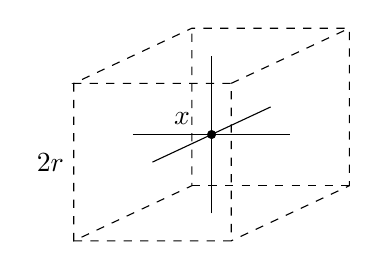
\begin{tikzpicture}
      \draw[dashed] (0,0)--(2,0)--(2,2)--(0,2)--(1.5,2.7)--(3.5,2.7)--(3.5,0.7)--(2,0);
      \draw[dashed] (2,2)--(3.5,2.7);
      \draw[dashed] (0,2)--(0,0)--(1.5,0.7)--(1.5,2.7);
      \draw[dashed] (1.5,0.7)--(3.5,0.7);
      \draw (1,1)--(2.5,1.7);
      \draw (0.75,1.35)--(2.75,1.35);
      \draw (1.75,0.35)--(1.75,2.35);
      \draw[fill] (1.75,1.35) circle (0.05);
      \node[above left] at (1.6,1.35) {$x$};
      \node[left] at (0,1) {$2r$};
  \end{tikzpicture}
  \end{center}

  The next theorem gives us a metric that induces the product topology on infinite dimensional $\mathbb{R}^\omega$ by slightly modifying the uniform metric on $\mathbb{R}$. However, with the box topology $\mathbb{R}^\omega$ is not metrizable. 

  \begin{theorem}
  Let $\Tilde{d} (a, b) \equiv \min{\{|a-b|, 1\}}$ be the standard bounded metric on $\mathbb{R}$. If $x, y \in \mathbb{R}^\omega$, we define
  \[ D(x, y) \equiv \sup{\Big\{ \frac{\Tilde{d}(x_i, y_i)}{i}\Big\}}\]
  Then, $D$ is a metric that induces the product topology on $\mathbb{R}^\omega$. 
  \end{theorem}
  It is easy to see that $0 \leq D(x, y) \leq 1$. So, given the open ball
  \[B_r (x) \equiv \{y \in \mathbb{R}^\omega \; | \; D(x, y) < r\}\]
  $B_r (x) = \mathbb{R}^\omega$ if $r > 1$. When $r \leq 1$, 
  \[B_r (x) \equiv (y-r, y+r) \times (y-2r, y+2r) \times ... = \prod_{k=1}^\infty (y - k r , y + k r)\]
  Visually, we take a cross section of this box and look at the slice within $\mathbb{R}_1 \times \mathbb{R}_2$, where the subscripts represent the first and second terms of $x$. 
  \begin{center}
  \begin{tikzpicture}
      \node[below left] at (0,0) {$y$};
      \draw[fill] (0,0) circle (0.05);
      \draw[<->] (0, -2)--(0,2);
      \draw[<->] (-3,0)--(3,0);
      \draw[fill] (-2,0) circle (0.05); 
      \draw[fill] (2,0) circle (0.05); 
      \draw[fill] (0,1) circle (0.05); 
      \draw[fill] (0,-1) circle (0.05); 
      \node[above left] at (-2,0) {$-2$};
      \node[above right] at (2,0) {$2$};
      \node[above right] at (0,1) {$1$};
      \node[below right] at (0,-1) {$-1$};
      \draw[fill] (0, 0.7) circle (0.05);
      \draw[fill] (1.4, 0) circle (0.05);
      \node[above left] at (0,0.7) {$r$};
      \node[below right] at (1.4,0) {$2r$};
      \draw[dashed] (-1.4, -0.7) rectangle (1.4,0.7);
      \node[right] at (0,2) {$\mathbb{R}_1$};
      \node[above] at (3,0) {$\mathbb{R}_2$};
  \end{tikzpicture}
  \end{center}

  \begin{proposition}
  Every metric topology satisfies the Hausdorff Axiom.
  \end{proposition}
  \begin{proof}
  If $x$ and $y$ are distinct points of $(X, d)$, then letting
  \[\varepsilon = \frac{1}{2} d(x, y)\]
  the triangle inequality implies that $B_\varepsilon (x)$ and $B_\varepsilon (y)$ are disjoint. 
  \end{proof}

  We now define continuity with the metric using the $\epsilon - \delta$ definition and connect it to the topological definition of continuity. Given 2 metric spaces $(X, d)$ and $(Y, \rho)$ with $f: X \longrightarrow Y$, it is clear that $x, y \in X \implies f(x), f(y) \in Y$. Given that $d(x, y) < \delta$ for a certain $\delta$, we can guarantee that $\rho(f(x), f(y)) < \epsilon$ for some $\epsilon$. In fact, we can make $\epsilon$ as small as we wish, and there will always be a $\delta > 0$ that satisfies $d(x, y) < \delta \implies \rho(f(x), f(y)) < \epsilon$.  

  \begin{definition}
  A function $f: (X, d) \longrightarrow (Y, \rho)$ between metric spaces is continuous at $p$ if for all $\epsilon > 0$, there exists a $\delta > 0$ such that 
  \[ d(x, p) < \delta \implies \rho ( f(x), f(p)) < \epsilon\]
  If $f$ is continuous at all $p \in X$, then we can say that $f$ is continuous.
  \end{definition}

  \begin{theorem}
  Now, we endow $(X, d), (Y, \rho)$ their open ball topologies, leading to the sets $(X, \tau_X, d)$ and $(Y, \tau_Y, \rho)$, respectively. Given function $f: X \longrightarrow Y$, we claim that $f$ is continuous according to the $\epsilon - \delta$ definition if and only if $f^{-1}(U) \in \tau_{X}$ for any $U \in \tau_Y$. That is, these two definitions of continuity are equivalent. 
  \end{theorem}

  \begin{proof}
  ($\rightarrow$) Assume $f$ is continuous according to the $\epsilon - \delta$ definition. Let $U$ be any open set in $Y$ containing the point $y$, and let $x$ be an element in $f^{-1}(U)$ such that $y = f(x)$. We must prove that $f^{-1}(U)$ is also open. Since open sets contain neighborhoods (e.g. open balls) of all of its points, we can claim that, since $U$ is open by assumption, there exists an open ball $B_y$ around $y$ with radius $\epsilon > 0$. This guarantees the existence of a point $z \in U$ such that $\rho(y, z) < \epsilon$ for any $\epsilon > 0$ that we choose. Since $f$ is continuous, for every $\epsilon >0$ that we chose previously, there exists a $\delta >0$ such that $d(x, w) \implies \rho(f(x), f(w)) < \epsilon$. Since $\rho(f(x), f(w)) < \epsilon$, we can conclude that $f(w) \in B_y \subset U$ when $d(x, w) < \delta$. Therefore, $d(x, w) < \delta \implies w \in f^{-1}(U)$. But this is equivalent to saying that if $w \in B_(x, \delta)$, then $w \in f^{-1}(U)$, which means that every single point $x \in f^{-1}(U)$ contains an open ball neighborhood fully contained in $f^{-1}(U)$. So, by definition, $f^{-1}(U)$ is open. 


  ($\leftarrow$) Assume $f^{-1}(U)$ is open when $U$ is an open set in $Y$, i.e. $f$ is continuous under the topological definition. Let us define the open ball 
  \[ B(f(x), \epsilon) \equiv \{ y \in Y \; | \; \rho(f(x), y) < \epsilon\} \in \tau_Y\]
  By our assumption, $f^{-1} \big( B(f(x), \epsilon) \big)$ is an open set in $\tau_X$, and clearly, $x \in f^{-1} \big( B(f(x), \epsilon) \big)$ since $f^{-1}$ maps the point $f(x) \in B(f(x), \epsilon)$ to $x \in f^{-1} \big( B(f(x), \epsilon) \big)$. But since $f^{-1} \big( B(f(x), \epsilon) \big)$ is open, we can construct an open ball around $x$ with radius $\delta$ fully contained within the open set. Moreover, by selecting a point $p \in B(f(x), \delta) \subset f^{-1}\big( B(f(x), \epsilon) \big)$, we can guarantee that $f(p) \in B(f(x), \epsilon)$. This is precisely the $\epsilon - \delta$ definition of continuity. That is, given an $\epsilon > 0$ to be the radius of an open ball $B(f(x), \epsilon)$ in $Y$, we can always choose a $\delta > 0$ to be the radius of the open ball $B(x, \delta)$ in $X$ that is fully contained within the preimage of $B(f(x), \epsilon)$. In mathematical notation, 
  \[ p \in B(x, \delta) \subset f^{-1} \big( B(f(x), \epsilon) \big) \implies f(p) \in f\big( B(x, \delta) \big) \subset B(f(x), \epsilon)\]
  or equivalently in terms of metrics,
  \[ d(x, p) < \delta \implies \rho (f(x), f(p)) < \epsilon\]
  \end{proof} 

  \begin{definition}
  A sequence $(x_\alpha)$ of points in topological space $(X, \mathscr{T})$ is said to \textbf{converge} to the point $x \in X$ if for every neighborhood $U$ of $x$ there exists a $N \in \mathbb{N}$ such that
  \[x_n \in U \text{ for all } n \geq N\]
  Furthermore, if a sequence converges, it converges to one point provided that $X$ is Hausdorff! For if $(x_\alpha)$ converges to $x$ and if $y \neq x$, then we need only choose disjoint neighborhoods of $y$ and $x$ to prove that $(x_\alpha)$, by definition, is not convergent to $y$.
  \end{definition}

  Visually, we can think of each $x_N$ in the sequence as a point in a metric space $(X, d)$. To see if $\{ x_i \}$ converges to a point $l \in X$, we construct an open ball $B(l, \epsilon)$ and see if all points $x_i$ after a certain $i = m$ lie within $B (l, \epsilon)$. If this can be done for all $\epsilon > 0$, then $\{ x_i \}$ converges to $l$, or 
  \[\lim_{i \to \infty} \{ x_i \} = l \]

  \begin{example}
  The space $(0,1)$ with the nested interval topology is not Hausdorff. In fact, it is impossible to distinguish 2 points $x, y$ if $x, y \in (0, \frac{1}{2})$, meaning that the sequence
  \[\frac{1}{10}, \frac{2}{10}, \frac{1}{10}, ...\]
  converges to both $\frac{1}{10}$ and $\frac{2}{10}$.
  \end{example} 

  We can extend the applications of the Bolzano Weierstrass Lemma from analysis to metric spaces in general with the following lemma. 

  \begin{lemma}[Sequence Lemma]
  If $X$ be a topological space with $A \subset X$. If there exists a sequence of points of $A$ that converges to $x$, then $x \in \bar{A}$. The converse is true if $X$ is metrizable. 
  \end{lemma}
  \begin{proof}
  $(\rightarrow)$ Our hypothesis says that $x$ is a limit point of $A$, which by definition means that $x \in \bar{A}$. \\
  $(\leftarrow)$ Assuming $X$ is metrizable and $x \in \bar{A}$, let $d$ be a metric for the topology of $X$. Then, for every $n \in \mathbb{N}$, let us define a sequence of open neighborhoods of $x$ to be
  \[\big(B_{\frac{1}{n}} (x) \big)\]
  Since $x \in \bar{A}$, there exists a point 
  \[x_n \in A \cap B_{\frac{1}{n}} (x) \text{ for all } n \in \mathbb{N}\]
  This sequence $(x_n)$ that we have proved must exist converges to $x$. 
  \end{proof}

  \begin{theorem}
  Let $f: X \longrightarrow Y$ and let $X$ be metrizable. $f$ is continuous if and only if for every convergent sequence $(x_n) \rightarrow x$ of $X$, the following sequence of $Y$ converges to $f(x)$. That is, 
  \[\big( f(x_n) \big) \longrightarrow f(x)\]
  \end{theorem}

  We introduce additional methods of constructing continuous functions. 

  \begin{lemma}
  The addition, subtraction, and multiplication operations are continuous functions from $\mathbb{R} \times \mathbb{R} \longrightarrow \mathbb{R}$, and the quotient operation is a continuous function from $\mathbb{R} \times (\mathbb{R} \setminus \{0\}) \longrightarrow \mathbb{R}$. 
  \end{lemma}
  \begin{proof}
  Standard $\epsilon-\delta$ proof. 
  \end{proof}

  \begin{theorem}
  If $X$ is a topological space, and if $f, g: X \longrightarrow \mathbb{R}$ are continuous, then $f + g$, $f-g$, and $f \cdot g$ are also continuous. $f / g$ is continuous if $g(x) \neq 0$ for all $x \in X$. 
  \end{theorem}

  \begin{definition}
  Let $f_n: X \longrightarrow Y$ be a sequence of functions from the set $X$ to the metric space $(Y, d)$. The sequence $(f_n)$ is said to \textbf{converge uniformly} to the function $f: X \longrightarrow Y$ if, given $\epsilon > 0$, there exists a $N \in \mathbb{N}$ such that
  \[d\big( f_n(x), f(x)\big) < \epsilon\]
  for all $n \geq N$ and for all $x \in X$. 
  \end{definition}

  \begin{theorem}[Uniform Limit Theorem]
  Let $f_n: X \longrightarrow Y$ be a sequence of continuous functions from topological space $X$ to a metric space $Y$. If $f_n$ converges uniformly to $f$, then $f$ is continuous. 
  \end{theorem}
  \begin{proof}
  $(\rightarrow)$ Trivial. \\
  $(\leftarrow)$ Let $V$ be open in $Y$, and let $x_0$ be a point in $f^{-1} (V)$. It suffices to prove that for every $x_0 \in f^{-1} (V)$, there exists a neighborhood $U$ of $x_0$ such that $U \subset F^{-1} (V)$ or equivalently, $F(U) \subset V$. 

  Let $y_0 = f(x_0)$. Since $Y$ is a metric space with metric $d$, we know that there exists an $\epsilon$-ball $B_\epsilon (y_0)$ such that
  \[B_\epsilon (y_0) \subset V\]
  Then, using uniform convergence, we can choose $N \in \mathbb{N}$ such that for all $n \geq N$ and all $x \in X$, 
  \[d \big( f_n (x), f(x) \big) < \frac{\epsilon}{4}\]
  which also applies at the point $x = x_0$. 
  \[d \big( f_n (x_0), f(x_0) \big) < \frac{\epsilon}{4}\]
  Using continuity of $f_n$, choose a neighborhood $U$ of $x_0$ such that $f_n$ carries $U$ into the open $\epsilon/2$-ball centered at $f_n (x_0)$ (note that $f_n (x_0) \neq y_0$), meaning that if $x \in U$
  \[d \big( f_n (x), f_n (x_0) \big) < \frac{\epsilon}{2}\]
  Adding the three inequalities and using the triangle inequality, we get the fact that if $x \in U$, then 
  \[d \big( f(x), f(x_0) \big) < \epsilon\]
  meaning that the $f(U) \subset B_\epsilon (x_0) \subset V$. 
  \end{proof}

  Visually, the three inequalities represent the following open balls in $V \subset Y$.
  \begin{center}
  \begin{tikzpicture}[scale=0.6]
      \draw[dashed, teal] (0,0) circle [radius=8];
      \draw[fill] (0,0) circle [radius=0.05];
      \draw[fill] (-1.5,0.5) circle [radius=0.05];
      \draw[dashed, purple] (0,0) circle [radius=2];
      \draw[dashed, purple] (-1.5,0.5) circle [radius=2];
      \node[right] at (0.3,0) {$f(x_0)$};
      \node[above right] at (-1.5,0.5) {$f_N (x_0)$};
      \draw[dashed, blue] (-1.5,0.5) circle [radius=4];
      \draw[fill] (-4,3) circle [radius=0.05];
      \draw[dashed, purple] (-4,3) circle [radius=2];
      \node[right] at (-4,3) {$f_N (x)$};
      \draw[fill] (-5.5, 3.7) circle [radius=0.05];
      \node[above left] at (-5,4.5) {$f(x)$};
      \draw[-, thick] (-5.5, 3.7)--(-4,3)--(-1.5,0.5)--(0,0);
      \draw[->, thick, purple] (0,0)--(0,-2);
      \draw[->, thick, blue] (-1.5,0.5)--(-1.5,-3.5);
      \node[right, purple] at (0,-1) {$\epsilon / 4$};
      \node[left,blue] at (-1.5,-1.5) {$\epsilon / 2$};
      \draw[->, thick, teal] (0,0)--(6.128, 5.1416);
      \node[below right, teal] at (3.064, 2.57) {$\epsilon$};
  \end{tikzpicture}
  \end{center}

  \begin{proposition}
  In a metric space $(X, d)$, a set is \textbf{closed} if the limit of every convergent subsequence in $X$ lies in $X$. That is, $X$ contains all of its limit points. 
  \end{proposition}

\section{Connectedness} 

    We briefly define some weaker forms of separability. Note that a space being $t_2$-separable is the condition of being Hausdorff. 

    \begin{definition}[$t_0, t_1$-Separability]
    Two points $x_1, x_2 \in X$ with topology $\tau_{X}$ is called $t_0$\textbf{-separable} if we can distinguish $x_1, x_2$ using open sets, i.e. if we can find an open set that contains $x_1$, but not $x_2$. A space $X$ with the property that any two distinct points in $X$ being $t_0$-separable is called a $t_0$-separable space. This is the weakest form of separability. 

    The next level of separability is called $t_1$-separability. When given 2 distinct points $x_1, x_2$ in $t_1$-separable set $X$, we can find neighborhoods $U_{x_1}, U_{x_2}$ such that $U_{x_1} \neq U_{x_2}$. 
    \begin{center}
        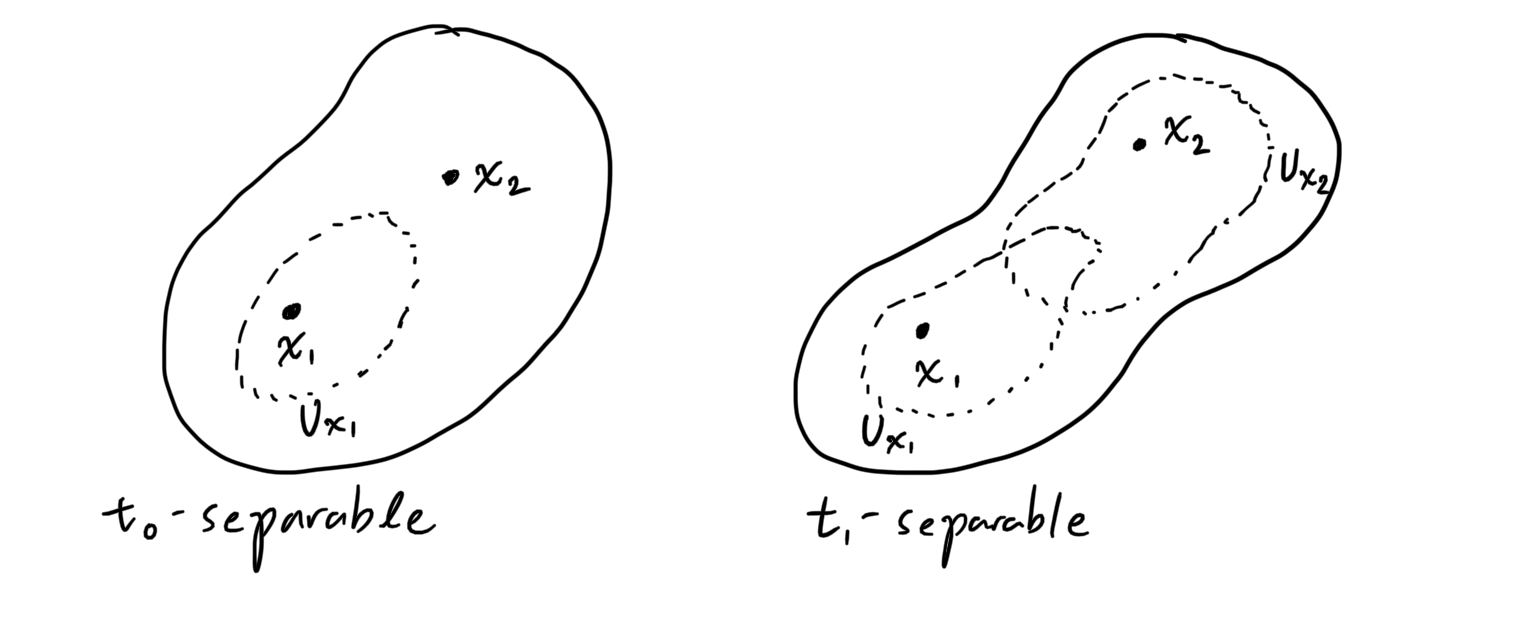
\includegraphics[scale=0.25]{img/t0_t1_Separability.PNG}
    \end{center}
    \end{definition}

    \begin{example}
    $(0,1)$ with the nested interval topology is not $t_0$-separable, since we can't distinguish $\frac{1}{4}$ and $\frac{1}{3}$.
    \end{example}

    \begin{example}
    $(0,1)$ with the cofinite topology is $t_0$-separable, since given distinct $x_1, x_2 \in (0,1)$, we can see that $x_1 \in X \setminus {x_2}$ and $x_2 \in X \setminus {x_1}$, which are both elements of the cofinite topology. By existence of these elements, $(0,1)$ is $t_1$-separable. 
    \end{example}

  \subsection{Connected Spaces}

    \begin{definition}
    Let $X$ be a topological space. A \textbf{separation} of $X$ is a pair $U, V$ of disjoint nonempty open subsets of $X$ whose union is $X$. The space $X$ is said to be \textbf{connected} if there does not exist a separation of $X$. 

    The visual below shows two examples of spaces that are not connected. 
    \begin{center}
        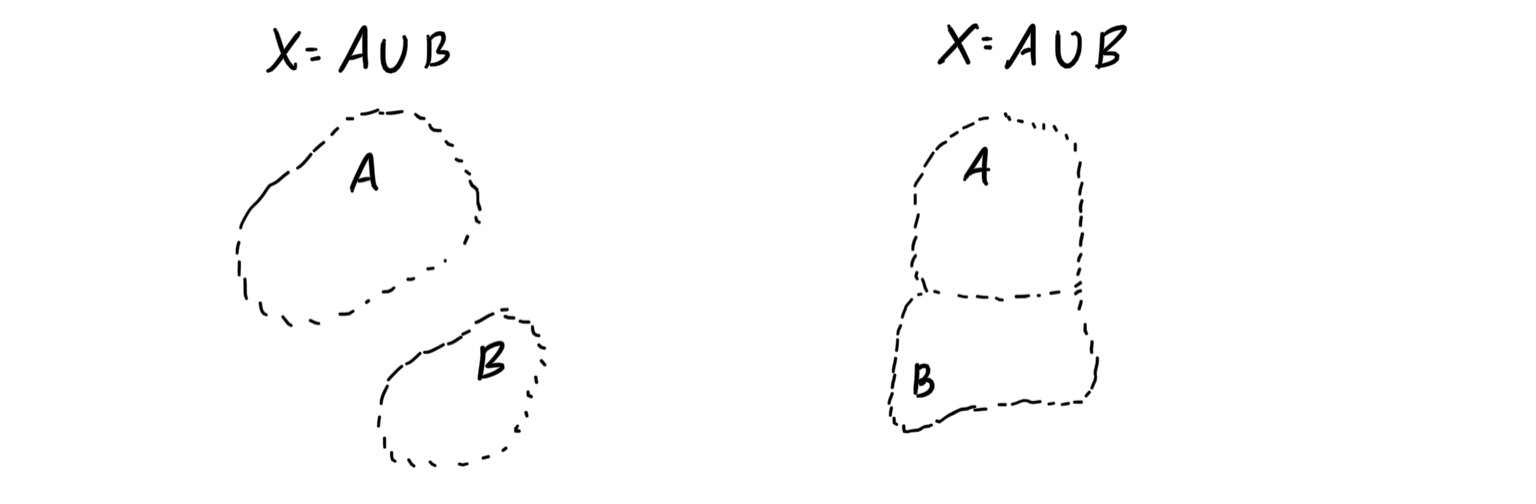
\includegraphics[scale=0.25]{img/Not_Connected_Spaces_Examples.PNG}
    \end{center}
    \end{definition}

    Connectedness is clearly a topological property since it is completely defined in terms of the collection of open sets in $X$. Since homeomorphisms preserves topological properties, we can say that if $X$ is connected, every space homeomorphic to $X$ is also connected. It is easy to see why the following definition of connectedness is equivalent to the first one. 

    \begin{definition}
    A space $X$ is \textbf{connected} if and only if the only subsets of $X$ that are clopen in $X$ are the empty set and $X$ itself. 
    \end{definition}

    \begin{lemma}
    If $Y$ is a subapce of $X$, a separation of $Y$ is a pair of disjoint nomempty sets $A$ and $B$ whose union is $Y$, neither of which contains a limit point of the other. The space $Y$ is connected if there exists no separation of $Y$. 
    \end{lemma}
    \begin{example}
    In the space $Y = (0,1) \times (0,1) \cup (1,2) \times (0,1) \subset \mathbb{R}^2$, we can visualize the separation of $Y$ as
    \begin{center}
    \begin{tikzpicture}[scale=1.5]
        \draw[dashed] (0,0) rectangle (2,1);
        \draw[dashed] (1,1)--(1,0);
    \end{tikzpicture}
    \end{center}
    Note that the dashed line is not in $Y$. Even though the dashed line contains limit points of both the left and right subset of $Y$, this does not matter. 
    \end{example}


    \begin{example}
    Let $X$ denote a two-point space in the indiscrete topology. Clearly, there is no separation of $X$, so $X$ is connected. 
    \end{example}

    \begin{example}
    Let $Y$ denote the subspace $[-1,0) \cup (0,1]$ of $\mathbb{R}$. Each of the sets $[-1,0)$ and $(0,1]$ is nonempty and open in $Y$ (but not in $\mathbb{R}$), so they form a separation of $Y$. Also, note that neither of these sets contains a limit point of the other (even though they have a common limit point $0$). 
    \end{example}

    \begin{example}
    $[-1,1]$, the subspace of $\mathbb{R}$, has no separation, so it is connected. 
    \end{example}

    \begin{example}
    The rationals $\mathbb{Q} \subset \mathbb{R}$ are not connected since given any irrational number $a$, we can write $Y$ as the union of sets
    \[Y \cap (-\infty, a), \; Y \cap (a, +\infty)\]
    which are open in the subspace topology. 
    \end{example}

    \begin{lemma}
    If the sets $C$ and $D$ form a separation of $X$, and if $Y$ is a connected subset of $X$, then $Y$ lies entirely within either $C$ or $D$. 
    \end{lemma}
    \begin{proof}
    Trivial. Easy to visualize. 
    \end{proof}

    \begin{theorem}
    The union of a collection of connected sets that have a point in common is connected. 
    \end{theorem}
    \begin{center}
    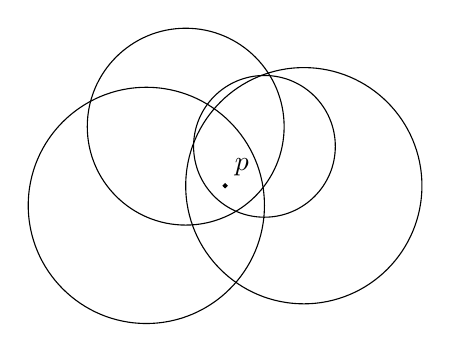
\begin{tikzpicture}[scale=0.5]
        \draw[fill] (0,0) circle (0.05);
        \node[above right] at (0,0) {$p$};
        \draw (1,1) circle (1.8);
        \draw (-1,1.5) circle (2.5);
        \draw (-2, -0.5) circle (3);
        \draw (2,0) circle (3);
    \end{tikzpicture}
    \end{center}

    \begin{proof}
    Let $\{A_\alpha\}$ be a collection of connected subsets of a space $X$, and let 
    \[p \in \bigcap A_\alpha\]
    Then, we claim that 
    \[Y \equiv \bigcup A_\alpha\]
    is connected. Assume $Y$ is not connected, that is, there exists $Y = C \cup D$ as a separation of $Y$. Then, $p \in C$ or $p \in D$. Without loss of generality, suppose $p \in C$. Since each $A_\alpha$ is connected, it must lie entirely within $C$ (by the previous lemma, since it contains the point $p \in C$) $\implies D = \emptyset$, a contradiction that $D$ must be nonempty. 
    \end{proof}

    \begin{theorem}
    Let $A$ be a connected subset of $X$. If $A \subset B \subset \bar{A}$, then $B$ is also connected. 
    \end{theorem}
    \begin{proof}
    Assume $B = C \cup D$ is a separation of $B \implies A$ must lie entirely within $C$ or $D$. Without loss of generality, suppose $A \subset C$, which implies that $\bar{A} \subset \bar{C}$. Since $\bar{C}$ and $D$ are disjoint, $B$ cannot intersect $D \implies D = \emptyset$, a contradiction. Therefore, there exists no separation of $B$. 
    \end{proof}

    \begin{theorem}
    The image of a connected space under a continuous map is connected. 
    \end{theorem}
    \begin{proof}
    Let $f: X \longrightarrow Y$ be a continuous map, and let $X$ be connected. We wish to prove that the image set $Z = f(X)$ is also connected. Let us denote the restriction of $f$ to $Z$ as
    \[\Tilde{f}: X \longrightarrow Z\]
    which is continuous and surjective. We prove by contradiction. Assume that $Z = A \cup B$ is a separation of $Z$ into 2 disjoint nonempty open sets. Then, $\Tilde{f}^{-1} (A)$ and $\Tilde{f}^{-1}(B)$ are disjoint open sets whose union is $X \implies \Tilde{f}^{-1} (A) \cup \Tilde{f}^{-1}(B)$ form a separation of $X$. This contradicts the hypothesis that $X$ is connected $\implies Z$ is connected.  
    \end{proof}

    \begin{theorem}
    Given connected topological spaces $X_\alpha$ with $\alpha \in J$, the Cartesian products of them is connected. That is, 
    \[\prod_{\alpha \in J} X_\alpha\]
    with the product topology is connected. If $J$ is infinite, then the product space is not necessarily connected under the box topology. 
    \end{theorem}

    \begin{definition}
    A simply ordered set $L$ having more than one element is called a \textbf{linear continuum} if the following hold. 
    \begin{enumerate}
        \item $L$ has the least upper bound property. 
        \item If $x <y$, then there exists $z$ such that $x<z<y$
    \end{enumerate}
    A classic example of the linear continuum is the real number line and every set homeomorphic to it. 
    \end{definition}

    \begin{theorem}
    If $L$ is a linear continuum in the order topology, then $L$ is connected and so it every interval and ray in $L$. 
    \end{theorem}

    \begin{corollary}
    $\mathbb{R}$ is connected, along with every interval and ray in $\mathbb{R}$. 
    \end{corollary}

    \begin{theorem}[Intermediate Value Theorem]
    Let $f: X \longrightarrow Y$ be a continuous map of the connected space $X$ into the ordered set $Y$, with the order topology. Given $a, b \in X$ and $r \in Y$ such that $f(a)<r<f(b)$, then there exists a point $c \in X$ such that $f(c) = r$. 
    \end{theorem}
    \begin{proof}
    Assuming the hypothesis, the sets 
    \[A \equiv f(X) \cap (-\infty, r), \; B \equiv f(X) \cap (r, +\infty)\]
    are disjoint. They are also nonempty since 
    \[f(a) \in A, \; f(b) \in B\]
    $A$ and $B$ are open since they are the intersection of open sets. Now, assume that there exists no point $c \in X$ such that $f(c) = r$. Then, 
    \[f(X) = A \cup B\]
    would define a separation of $X$, contradicting the fact that the image of a connected space under a continuous map must be connected. Therefore, $c$ exists. 
    \end{proof}

    \begin{definition}
    Given points $x$ and $y$ of the space $x$, a \textbf{path} in $X$ from $x$ to $y$ is a continuous map $f: [a,b] \longrightarrow X$ of some closed interval in $\mathbb{R}$ to $X$ such that $f(a) = x$ and $f(b)=y$. A space $X$ is said to be \textbf{path connected} if every pair of points of $X$ can be joined by a path in $X$. 
    \end{definition}

    \begin{proposition}
    $X$ is path connected $\implies X$ is connected. 
    \end{proposition}
    \begin{proof}
    $X$ not connected implies that there exists disjoint open subsets $C, D$ such that $C \cup D = X$. Assume that $X$ is path connected, i.e. there exists a continuous function $g: [0,1] \longrightarrow X$. Then the preimage of $C$ and $D$ in $X$ must be open sets $g^{-1} (C), g^{-1} (D) \subset [0,1]$ such that $g^{-1}(C) \cup g^{-1}(D) = [0,1]$. But this isn't possible since $[0,1]$ is connected, so by contradiction, $X$ is not path connected. The contrapositive of this statement results in the proposition. 
    \end{proof}

    \begin{center}
    \begin{tikzpicture}[scale=0.5]
        \draw[dashed] (5,1) circle (2);
        \draw[dashed] (0,0) circle (2);
        \node at (-1,-1) {$C$};
        \node at (6,2) {$D$};
        \draw plot [smooth] coordinates {(0,0) (2,1.5) (4.5,2)};
        \draw[fill] (0,0) circle (0.05);
        \draw[fill] (4.5,2) circle (0.05);
        \node at (-4,1) {$X = C \cup D$};
    \end{tikzpicture}
    \end{center}

    However, note that $X$ connected $\centernot\implies$ $X$ path connected. Note the following example. 

    \begin{example}
    \[ f:[0,1] \longrightarrow [-1,1], \; f(x) = \sin{\frac{1}{x}}\]
    $[-1,1]$ is connected, but not path connected since the path oscillates infinitely many times as it approaches $0$ from both $-1$ and $1$. 
    \end{example}

    The concept of homotopies is dealt with in algebraic topology, but it is worthwhile to mention it now. 

    \begin{definition}
    Two continuous paths from $x$ to $y$ in topological space $X$ is \textbf{homotopic} if one can be continuously "deformed" into the other, such a deformation being the \textbf{homotopy} between two functions. The set of linearly homotopic paths form a relation, and thus \textbf{homotopy classes} can be further defined. 
    \end{definition}

    Visually, the set of all the curves in the space $X$ as shown are in a single homotopy class.
    \begin{center}
    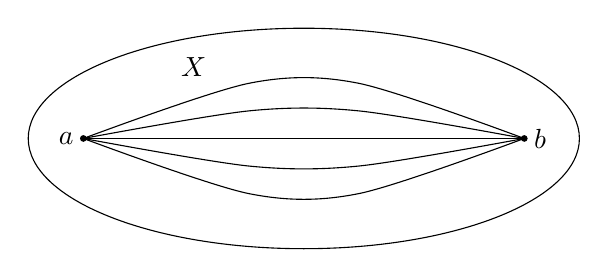
\begin{tikzpicture}[scale=0.7]
        \draw (0,0) ellipse (5 and 2);
        \draw[fill] (-4,0) circle (0.05);
        \draw[fill] (4,0) circle (0.05);
        \draw plot [smooth] coordinates {(-4,0) (-1,1) (1,1) (4,0)};
        \draw (-4,0)--(4,0);
        \draw plot [smooth] coordinates {(-4,0) (-1,0.5) (1,0.5) (4,0)};
        \draw plot [smooth] coordinates {(-4,0) (-1,-0.5) (1,-0.5) (4,0)};
        \draw plot [smooth] coordinates {(-4,0) (-1,-1) (1,-1) (4,0)};
        \node at (-2,1.3) {$X$};
        \node[left] at (-4,0) {$a$};
        \node[right] at (4,0) {$b$};
    \end{tikzpicture}
    \end{center}
    It is clear that the space $X$ consists of a single homotopy class of curves from $a$ to $b$. However, let us define the space $Y \equiv X \setminus C$ where $C$ is a circular region in $X$. Then, $Y$ has an infinite number of homotopy classes. We show two curves, that are in two different homotopy classes. 
    \begin{center}
    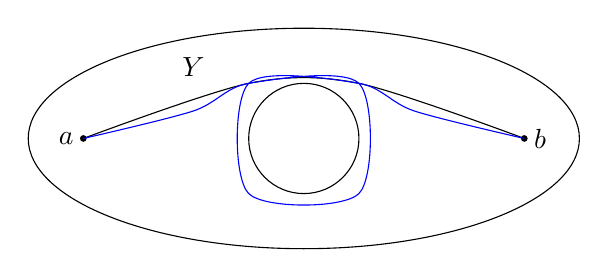
\begin{tikzpicture}[scale=0.7]
        \draw (0,0) ellipse (5 and 2);
        \draw[fill] (-4,0) circle (0.05);
        \draw[fill] (4,0) circle (0.05);
        \draw plot [smooth] coordinates {(-4,0) (-1,1) (1,1) (4,0)};
        \node[left] at (-4,0) {$a$};
        \node[right] at (4,0) {$b$};
        \draw (0,0) circle (1);
        \node at (-2,1.3) {$Y$};
        \draw[blue] plot [smooth] coordinates {(-4,0) (-2,0.5) (-1,1) (1,1) (1,-1) (-1,-1) (-1,1) (1,1) (2,0.5) (4,0)};
    \end{tikzpicture}
    \end{center}

    \begin{definition}
    A \textbf{simply connected set} is a set such that all paths between any two given points are homotopic. That is, a simply connected set has one homotopy class. 
    \end{definition}

  \subsection{Components and Path Components}

    \begin{definition}
    Given $X$, define an equivalance relation on $X$ by setting $x \sim y$ if there is a connected subset of $X$ containing both $x$ and $y$. The equivalence classes are called the \textbf{components}, or \textbf{connected components}, of $X$. 
    \end{definition}

    \begin{theorem}
    The components of $X$ are connected disjoint subsets of $X$ whose union is $X$, such that each connected subset of $X$ intersects only one of them. 
    \end{theorem}
    \begin{proof}
    Trivial. 
    \end{proof}

    \begin{definition}
    We can define another equivalence relation on the space $X$ by defining $x \sim y$ if there is a path in $X$ from $x$ to $y$. The equivalence classes are called the \textbf{path components} of $X$. It can be easily shown that this is an equivalence relation. 
    \end{definition}

    \begin{theorem}
    The path components of $X$ are path connected disjoint subsets of $X$ whose union is $X$, such that each path connected subset of $X$ intersects only one of them. 
    \end{theorem}
    \begin{proof}
    Trivial.
    \end{proof}

    The property of local connectedness is also important for a space to possess. Roughly speaking, local connectivity means that each point has "arbitrarily small" neighborhoods that are connected. 

    \begin{definition}
    A space $X$ is said to be \textbf{locally connected at $x$} if for every neighborhood $U$ of $x$, there is a connected open neighborhood $V$ of $x$ contained in $U$. If $X$ is locally connected at all of its points, then $X$ is simply said to be \textbf{locally connected}. 
    \end{definition}
    Visually, in the space $X$, let $U$ be the union of the two open balls shown below. $U$ is clearly open, but not necessarily connected. However, we can form a  neighborhood $V$ of $x$ contained in $U$ such that $V$ is connected. 
    \begin{center}
    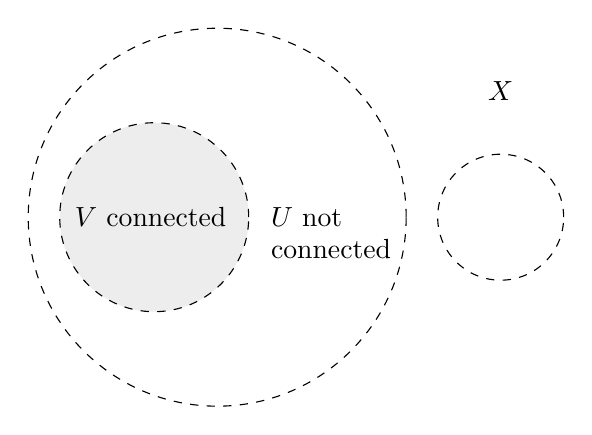
\begin{tikzpicture}[scale=0.8]
        \draw[fill] (-2,0) circle (0.05);
        \node[above] at (-2,0) {$x$};
        \draw[dashed] (-1.5,0) circle (3);
        \draw[dashed] (3,0) circle (1);
        \draw[dashed, fill=lightgray] (-2.5,0) circle (1.5);
        \node[left] at (-1.2,0) {$V$ connected};
        \node[right] at (-0.8,0) {$U$ not};
        \node[right] at (-0.8,-0.5) {connected};
        \node at (3,2) {$X$};
    \end{tikzpicture}
    \end{center}

    Equivalently, $X$ is locally connected if there exists a basis for $X$ consisting of connected sets. Local connectedness and connectedness of a space are independent of each other. 

    \begin{definition}
    A space $X$ is \textbf{locally path connected at $x$} if for every neighborhood $U$ of $x$, there is a path connected neighborhood $V$ of $x$ completely contained in $U$. If $X$ is locally path connected at each of its points, then it is simply said to be \textbf{locally path connected}. We can visualize this condition similarly as that of local connectedness. 
    \end{definition}

    \begin{theorem}
    A space $X$ is locally connected if and only if for every open set $U$ of $X$, each component of $U$ is open in $X$. 
    \end{theorem}
    \begin{proof}
    $(\rightarrow)$ Suppose that $X$ is locally connected. Let $U$ be an open set of $X$ and let $C$ be a component of $U$. If $x$ is any point in $C$, by definition of local connectedness, there exists a connected neighborhood $V$ of $x$ fully contained in $U$. Since $V$ is connected, it must additionally lie completely within $C \implies C$ is open in $X$. \\
    $(\leftarrow)$ Suppose that the components of open sets in $X$ are open. Given a point $x \in X$ and neighborhood $U$ of $x$, let $C$ be the component of $U$ containing $x$, which means that $C$ is connected. By hypothesis, the components of open sets are alsvo open, so $C$ is also open. Since an open, connected set $C$ exists for all $x \in X$, $X$ is locally connected. 
    \end{proof}

    \begin{theorem}
    A space $X$ is locally path connected if and only if for every open set $U$ of $X$, each path component of $U$ is open in $X$.
    \end{theorem}

    \begin{theorem}
    If $X$ is a topological space, each path component of $X$ lies in a component of $X$. If $X$ is locally path connected, then the components and the path components of $X$ are the same. 
    \end{theorem}

\section{Compact Spaces}

    \begin{definition}
    A collection $\mathscr{C}$ of subsets of a space $X$ is said to \textbf{cover} $X$, or to be a \textbf{covering} of $X$, if the union of the elements of $\mathscr{C}$ is equal to $X$. It is called an \textbf{open covering} of $X$ if its elements are open subsets of $X$. 
    \end{definition}

    \begin{definition}
    A space $X$ is said to be \textbf{compact} if every open covering of $X$ contains a finite subcovering (i.e. a finite collection of subcovers) of $X$. It may be better to think of compactness as such: If you can find any infinite open covering of the space, then it is not compact. 
    \end{definition}

    \begin{lemma}
    Let $Y$ be a subspace of $X$. Then $Y$ is compact if and only if every covering of $Y$ by sets open in $X$ contains a finite subcollection covering $Y$. 
    \end{lemma}

  \subsection{Intuition behind Compactness}

    The concept of compactness does not seem intuitive at first glance. The reason why compactness is such an important property for a space to have is because $X$ being compact tells us that we can \textbf{always} analyze the entire $X$ using a \textbf{finite} union of open sets, which can simplify the space greatly. That is, it a measure of finiteness of a space. 

    It is well known that the behavior of finite sets and infinite sets can be different. For example, the four statements below are easily seen to be true whenever $X$ is a finite set, but false whenever $X$ is an infinite set. 
    \begin{enumerate}
        \item (All functions are bounded) If $f: X \longrightarrow \mathbb{R}$ is a real valued function on $X$, then $f$ must be bounded. That is, there exists a finite number $M$ such that $|f(x)| \leq M$ for all $x \in X$. 
        \item (All functions attain a maximum) If $f: X \longrightarrow \mathbb{R}$ is a real-valued function on $X$, then there must exist at least one point $x_0 \in X$ such that $f(x_0) \geq f(x)$ for all $x \in X$. 
        \item (All sequences have constant subsequences) If $(x_\alpha)_{\alpha \in \mathbb{N}}$ is a sequence in $X$, then there must exist a subsequence $x_{\beta_1}, x_{\beta_2}, x_{\beta_3}, ...$ which is constant. That is, $x_{\beta_1} = x_{\beta_2} = x_{\beta_3} = \cdot = c$ for some $c \in X$. 
        \item (All covers have finite subcovers) If $V_1, V_2, V_3, \cdot \subset X$ are any collection of sets which cover $X$, then there must exist a finite sub-collection $V_{n_1}, V_{n_2}, ..., V_{n_k}$ of these sets which still cover $X$. 
    \end{enumerate}

    The fact that all functions on a finite set are bounded is an example of a \textbf{local-to-global principle}. Namely, the hypothesis is an assertion of "local" boundedness: it asserts that $|f(x)|$ is bounded for each point $x \in X$ separately (which can depend on $x$). This collection of local boundedness can be extrapolated to global boundedness: that $|f(x)|$ is bounded by a \textbf{single} bound $M$ for all $x \in X$. This local-to-global boundedness is clearly valid when $X$ is finite, but it fails when $X$ is finite. For example, consider the function
    \[id: \mathbb{N} \longrightarrow \mathbb{R}\]
    which is clearly not bounded by any finite element in $\mathbb{R}$. 

    However, given that we endow a metric or a topology on the set $X$, we can actually find some infinite sets that are "almost finite," in the way that they satisfy a modified version of these four assertions, which are created by introducing topological concepts such as continuity, convergence, and openness. One such "almost finite" set is the closed interval $[0,1]$. 
    \begin{enumerate}
        \item (All \textbf{continuous} functions are bounded) If $f: X \longrightarrow \mathbb{R}$ is a real-valued continuous function on $X$, then $f$ must be bounded. (This is another type of local-to-global principle; if a function is stable with respect to local perturbations, then it is stable with respect to global perturbations).
        \item (All \textbf{continuous functions} attain a maximum) If $f: X \longrightarrow \mathbb{R}$ is a real-valued continuous function on $X$, then there exists at least one point $x_0 \in X$ such that $f(x_0) \geq f(x)$ for all $x \in X$. 
        \item (All sequences have convergent subsequences) If $x_1, x_2, ... \in X$ is a sequence of points in $X$, then there must exist a subsequence $x_{n_1}, x_{n_2}, ...$ which is convergent to some limit $c \in X$. (Bolzano-Weierstrass theorem).
        \item (All open covers have finite subcovers) If $V_1, V_2, V_3, ... \subset X$ are any collection of open sets which cover $X$, then there must exist a finite subcollection $V_{n_1}, V_{n_2}, ..., V_{n_k}$ of these sets which still cover $X$. 
    \end{enumerate}

    However, the open interval $(0,1)$ clearly does not satisfy any of these properties. For example, the continuous function 
    \[f: (0,1) \longrightarrow \mathbb{R}, \; f(x) \equiv \frac{1}{1-x}\]
    does not satisfy the boundedness condition, meaning that it does not satisfy the local-to-global principle. That is, $f$ is not stable under local perturbations of $x$. As you can guess by now, these "almost finite" sets that satifies these "weakened" topological conditions are compact sets. 
    \[\begin{tikzcd}
    Compact \;Sets \arrow{r}{satisfies} & Compact \;Conditions \\
    Finite \;Sets \arrow{r}{satisfies} & Finite \;Conditions \arrow{u}{weakened}
    \end{tikzcd}\]

    However, the four properties are not exactly equivalent, so we can define compactness according to the fourth property: that every open cover has a finite subcover. There are other notions of compactness, such as \textbf{sequential compactness}, which is based on the third version: all sequences have convergent subsequences. 

    Compactness if a powerful property of spaces with many applications. One is via appeal to local-to-global principles; one establishes local control on some function or other quantity, and then uses compactness to boost the local control to global control. Another is to locate amaxima or minima of a function. Of course, many spaces of interest are not compact. For instance, the real line $\mathbb{R}$ is not compact because contains sequences such as $1, 2, 3, \cdot$ which are "trying to escape" the real line, and are not leaving behind and convergent subsequences. However, one can recover compactness by adding a few more points to the space, a process known as \textbf{compactification}. We can add one point at either end of the real line, at $+\infty$ and $-\infty$, resulting in the compact \textbf{extended real line}. 


    \begin{example}
    The subset $Y \equiv (0,1) \times (0,1) \subset \mathbb{R}^2$ is not compact. That is, we can choose to cover the subspace by the finite union of open sets. 
    \[[0,1]^2 \subset \bigcup_{k=0}^\infty \Big( \frac{2^k - 1}{2^k}, \frac{2^{k+1} - 1}{2^{k+1}} \Big) \times (0,1)\]
    We show the first three elements of the infinite union that covers the open square.  
    \begin{center}
    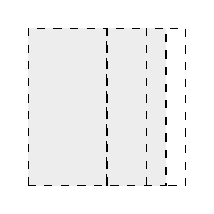
\begin{tikzpicture}[scale=2]
        \draw[dashed] (0,0) rectangle (1,1);
        \draw[dashed, fill=lightgray] (0,0) rectangle (0.5,1);
        \draw[dashed, fill=lightgray] (0.5,0) rectangle (0.75,1);
        \draw[dashed, fill=lightgray] (0.75,0) rectangle (0.875,1);
    \end{tikzpicture}
    \end{center}
    \end{example}

    \begin{theorem}
    Every closed subset of a compact space is compact. 
    \end{theorem}
    \begin{proof}
    This proof is quite trivial. Let $Y$ be a closed subset of compact space $X$. Given a covering $\mathcal{C}$ of $Y$ by sets open in $X$, let us form an open covering $\mathscr{B}$ of $X$ by adjoining to $\mathcal{C}$ the single open set $X \setminus Y$. Then, we an see that both $\mathscr{B}$ and $\mathcal{C} \cup (X \setminus Y)$ covers $X$. 
    \[\mathscr{B} = \mathcal{C} \cup (X \setminus Y)\]
    Since $\mathscr{B}$ is finite, the right hand side must also be expressible as a finite union. Looking through $\mathscr{B}$, we can throw away all the open sets that are entirely in $X \setminus Y$. What remains is a finite covering of $Y$. 
    \end{proof}

    \begin{theorem}
    Every compact subset of a Hausdorff space is closed. 
    \end{theorem}
    \begin{proof}
    Let $Y$ be a compact subset of the Hausdorff Space $X$. We claim that $X \setminus Y$ is open. Let $x \in X \setminus Y$. Then, for each point $y_i \in Y$, we can choose disjoint neighborhoods $U_i$ of $x$ and $V_i$ of $y_i$ (using the Hausdorff condition). The collection 
    \[\{V_i \; | \; y_i \in Y\}\]
    is an open covering $Y$. Since $Y$ is compact, there must exist a finite number of open sets $V_1, V_2, ..., V_n$ covering $Y$. Therefore, 
    \[\bigcup_{i=1}^n V_i\]
    contains $Y$ and is disjoint from the intersection of open neighborhoods of $x$
    \[U \equiv \bigcap_{i=1}^n U_i\]
    Therfore, $U$ is an open neighborhood of $x_0$, disjoint from $Y \implies X \setminus Y$ is open $\implies Y$ is closed.
    \end{proof}

    This results gives the following lemma. 

    \begin{lemma}
    If $Y$ is a compact subset of a Hausdorff space $X$ and $x_0$ is not in $Y$, then there exist disjoint open sets $U$ and $V$ of $X$ containing $x_0$ and $Y$, respectively. 
    \end{lemma}

    \begin{center}
    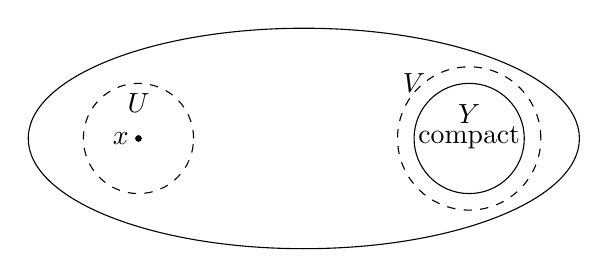
\begin{tikzpicture}[scale=0.7]
        \draw (0,0) ellipse (5 and 2);
        \draw[dashed] (-3,0) circle (1);
        \draw[fill] (-3,0) circle (0.05);
        \node[left] at (-3,0) {$x$};
        \draw (3,0) circle (1); 
        \node[below] at (3,0.8){$Y$};
        \node[below] at (3, 0.4){compact};
        \node[above] at (-3,0.3) {$U$};
        \draw[dashed] (3,0) circle (1.3); 
        \node at (2,1) {$V$};
    \end{tikzpicture}
    \end{center}

    \begin{theorem}
    The image of a compact space under a continuous map is compact.
    \end{theorem}
    \begin{proof}
    Let $f: X \longrightarrow Y$ be continuous, and let $X$ be compact. Let $\mathcal{C}$ be a covering of the set $f(X)$ by sets open in $Y$. Then, the preimage of these sets is the collection
    \[\{f^{-1}(\mathcal{A}) \; | \; \mathcal{A} \in \mathcal{C}\}\]
    which clearly covers $X$. But since $X$ is compact, a finite number of them, say
    \[f^{-1} (\mathcal{A}_1), f^{-1} (\mathcal{A}_2), ..., f^{-1} (\mathcal{A}_n)\]
    covers $X \implies \mathcal{A}_1, \mathcal{A}_2, ..., \mathcal{A}_n$ covers $f(X)$. 
    \end{proof}

    \begin{theorem}
    Let $f: X \longrightarrow Y$ be a bijective continuous function. If $X$ is compact and $Y$ is Hausdorff, then $f$ is a homeomorphism. 
    \end{theorem}
    \begin{proof}
    It suffices to prove that $f$ is an open or closed mapping. We shall show that $f$ is the latter. Let $U$ be closed in $X$. By the previous theorems, $U$ is compact $\implies f(U)$ is compact in Hausdorff $Y \implies f(U)$ is closed. Therefore, $f$ is closed. 
    \end{proof}

    We now introduce a useful lemma that will come around in many future cases. 

    \begin{lemma}[Tube Lemma]
    Consider the product space $X \times Y$, where $Y$ is compact. If $N$ is an open set $X \times Y$ containing the slice $x_0 \times Y$ of $X \times Y$, then $N$ contains some tube $W \times Y$ about $x_0 \times Y$, where $W$ is a neighborhood of $x_0$ in $X$. 
    \end{lemma}
    \begin{center}
    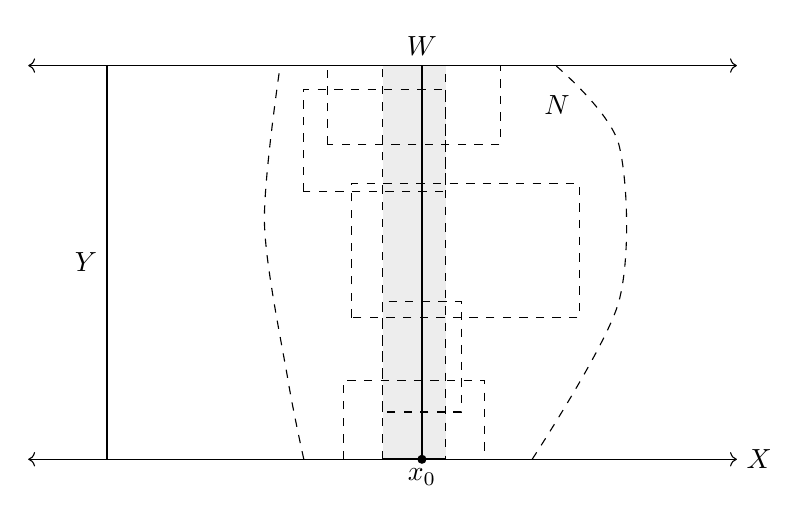
\begin{tikzpicture}
        \draw[dashed, fill=lightgray] (3.5,0) rectangle (4.3,5);
        \draw (0,0)--(0,5);
        \draw[<->] (-1,0)--(8,0);
        \node[right] at (8,0) {$X$};
        \node[left] at (0,2.5) {$Y$};
        \draw[<->] (-1,5)--(8,5);
        \draw[thick] (4,0)--(4,5);
        \draw[dashed] (3,0) rectangle (4.8,1);
        \draw[dashed] (3.5,0.6) rectangle (4.5,2);
        \draw[dashed] (3.1,1.8) rectangle (6,3.5);
        \draw[dashed] (2.5,3.4) rectangle (4.3,4.7);
        \draw[dashed] (2.8,4) rectangle (5, 5);
        \draw[thick] (3.5,0)--(4.3,0);
        \node[above] at (4,5) {$W$};
        \node[below] at (4,0) {$x_0$};
        \draw[fill] (4,0) circle (0.05);
        \draw[dashed] plot [smooth] coordinates {(2.5,0) (2.3, 1) (2,3) (2.2,5)};
        \draw[dashed] plot [smooth] coordinates {(5.4,0) (6.5,2) (6.5,4) (5.7,5)};
        \node[left] at (6,4.5) {$N$};
    \end{tikzpicture}
    \end{center}
    \begin{proof}
    Let us cover $x_0 \times Y$ by basis elements $U \times V$ (for the topology of $X \times Y$) lying in $N$. The space $x_0$ is compact since it is homeomorphic to $Y \implies$ we can cover $x_0 \times Y$ by finitely such basis elements
    \[U_1 \times V_1, U_2 \times V_2, ..., U_n \times V_n\]
    Without loss of generality, we can assume that each $U_i \times V_i$ has a nontrivial intersection with $x_0 \times Y$, since otherwise, it would be superfluous. Now, we define the intersection of all the open neighborhoods of $x_0$ in $X$ of the basis elements $U_i \times V_i$. That is, let
    \[W \equiv \bigcup_{i=1}^n U_i\]
    As an intersection of open sets, $W$ is also open containing $x_0$. With this well-defined tube $W \times Y$, we claim that it is entirely contained within $N$. That is, given a point $x \times y \in W \times Y$, consider the corresponding point $x_0 \times y$ that is the image of the projection of $x\times y$ onto $x_0 \times Y$. Clearly, $x_0 \times y$ belongs to some $U_k \times V_k$ (for some $k$) $\implies y \in V_k$. Since $x \in W$, $x$ is clearly in $U_k$, meaning that $x \times y \in U_k \times V_k \subset N$, as desired. 
    \end{proof}

    \begin{theorem}
    The product of finitely many compact spaces is compact. 
    \end{theorem}
    \begin{proof}
    Using induction, it suffices to prove that the product of 2 compact spaces is compact. Let $X$ and $Y$ be compact spaces. By the tube lemma, for each $x \in X$, there exists a neighborhood $W_x$ of $x$ such that the tube $W_x \times Y$ can be covered with finitely (by compactness of $Y$) many open sets in $X \times Y$. The collection of all neighborhoods $W_x$ is an open covering of $X$. By compactness of $X$, there exists a finite subcollection
    \[W_1, W_2, ..., W_k\]
    covering $X$. The finite union of the tubes 
    \[\bigcup_{i=1}^k W_i \times Y\]
    clearly covers $X \times Y$, meaning that $X \times Y$ is compact. 
    \end{proof}

    \begin{definition}
    A collection $\mathcal{C}$ of subsets of $X$ is said to satisfy the \textbf{finite intersection condition} if for every finite subcollection 
    \[\{\mathcal{C}_1, \mathcal{C}_2, ..., \mathcal{C}_n\}\]
    of $\mathcal{C}$, the intersection
    \[\bigcap_{i=1}^n \mathcal{C}_i\]
    is nonempty. 
    \end{definition}

    Clearly, the empty sets cannot below to any collection with the finite intersection property. Additionally, the condition is trivially satisfied if the intersection over the entire collection is non-empty or if the collection is nested. However, here is one example that does satisfy the finite intersection condition. 

    \begin{example}
    Let $X = (0,1)$ and for each positive integer $i$, $X_i$ is the set of elements of $X$ having a decimal expansion with digit $0$ in the $i$th decimal place. Then, any finite intersection of $X_i$'s is nonempty, but the intersection of all $X_i$ for $i \in \mathbb{N}$ is empty, since no element of $(0,1)$ has all zero digits. 
    \end{example}

    Here is an analogous example to the previous one. 
    \begin{example}
    In the space $\mathbb{R}$, let us define $C_i \equiv \mathbb{R} \setminus \{i\}$. That is, $C_i$ is $\mathbb{R}$ missing a point at $i$. Then, the collection of all $C_i$'s does satisfy the finite intersection condition. We show below the finite intersection of the five subsets $C_0, C_1, C_2, C_3, C_4$. 
    \begin{center}
    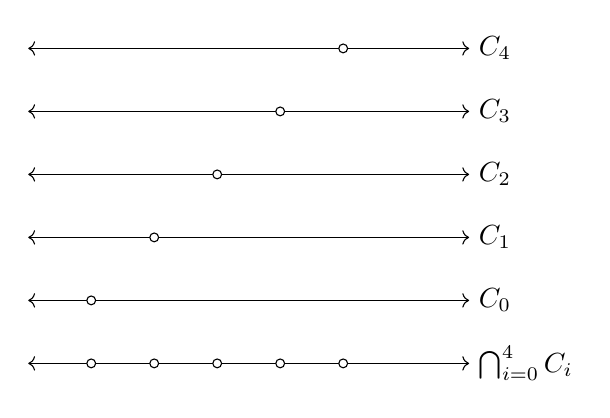
\begin{tikzpicture}[scale=0.8]
        \draw[<->] (-1,0)--(6,0);
        \draw[<->] (-1,1)--(6,1);
        \draw[<->] (-1,2)--(6,2);
        \draw[<->] (-1,3)--(6,3);
        \draw[<->] (-1,4)--(6,4);
        \draw[<->] (-1,-1)--(6,-1);
        \draw[fill=white] (0,0) circle (0.07); 
        \draw[fill=white] (1,1) circle (0.07); 
        \draw[fill=white] (2,2) circle (0.07); 
        \draw[fill=white] (3,3) circle (0.07); 
        \draw[fill=white] (4,4) circle (0.07); 
        \draw[fill=white] (0,-1) circle (0.07); 
        \draw[fill=white] (1,-1) circle (0.07); 
        \draw[fill=white] (2,-1) circle (0.07); 
        \draw[fill=white] (3,-1) circle (0.07); 
        \draw[fill=white] (4,-1) circle (0.07); 
        \node[right] at (6,-1) {$\bigcap_{i=0}^4 C_i$};
        \node[right] at (6,0) {$C_0$};
        \node[right] at (6,1) {$C_1$};
        \node[right] at (6,2) {$C_2$};
        \node[right] at (6,3) {$C_3$};
        \node[right] at (6,4) {$C_4$};
    \end{tikzpicture}
    \end{center}
    \end{example}


    \begin{theorem}
    Let $X$ be a topological space. Then $x$ is compact if and only if for any collection $\mathcal{C}$ of closed sets in $X$ satisfying the finite intersection condition, the intersection 
    \[\bigcap_{C \in \mathcal{C}} C\]
    of all the elements of $\mathcal{C}$ is nonempty. 
    \end{theorem}
    \begin{proof}
    Given a collection $S$ fo subets of $X$, let 
    \[\mathcal{C} \equiv \{X \setminus A \; | \; A \in S\}\]
    be the collection of their complements. Then, the following statements hold 
    \begin{enumerate}
        \item $S$ is a collection of open sets if and only if $\mathcal{C}$ is a collection of closed sets. 
        \item The collection $S$ covers $X$ if and only if the intersection 
        \[\bigcap_{C \in \mathcal{C}} C\]
        of all the elements of $\mathcal{C}$ is empty. 
        \item The finite subcollection $\{A_1, A_2, ..., A_n\}$ of $S$ covers $X$ if and only if the intersection of the corresponding elements $C_i \equiv X \setminus A$ of $\mathcal{C}$ is empty. 
    \end{enumerate}
    Clearly, (1) is trivial, and (2) and (3) follows from DeMorgan's Law. 
    \[X \setminus \bigcup_{\alpha \in J} A_\alpha = \bigcap_{\alpha \in J} (X \setminus A_\alpha)\]
    Using statement 3, the existence of a finite collection of closed sets $C$ in $X$ satisfying the finite intersection condition is equivalent to its complements (which are open sets) covering $X$, which is precisely the definition of compactness. 
    \end{proof}

    Clearly, the previous example in the real line $\mathbb{R}$ shows that $\mathbb{R}$ is indeed not compact. 

    \begin{corollary}
    The space $X$ is compact if and only if every collection $\mathscr{C}$ of subsets of $X$ satisfying the finite intersection condition, the intersection 
    \[\bigcap_{A \in \mathscr{C}} \bar{A}\]
    of their closures is nonempty. 
    \end{corollary}

  \subsection{Compact Sets of the Real Line}

    In order to construct new compact spaces from old ones, we must prove compactness for a number of fundamental spaces. The real number line is a good starting point, and in order to prove that every closed interval in $\mathbb{R}$ is compact, we only need the following theorem. 

    \begin{theorem}
    Let $X$ be a simply ordered set having the least upper bound property (That is, every nonempty subset of $X$ with an upper bound has a least upper bound). Then, in the order topology, every closed interval in $X$ is compact. 
    \end{theorem}

    \begin{corollary}
    Every closed interval in $\mathbb{R}$ is compact. 
    \end{corollary}

    \begin{theorem}[Heine-Borel Theorem]
    A subset $A$ of $\mathbb{R}^n$ is compact if and only if it is closed and bounded in the Euclidean metric $d$ or the square metric $p$. 
    \end{theorem}

    \begin{example}
    The unit sphere $S^{n-1}$ and the closed ball $B^n$ in $\mathbb{R}^n$ are compact since they are closed and bounded. The set
    \[A \equiv \{(x, \frac{1}{x}) \; | \; 0 < x \leq 1\}\]
    is closed in $\mathbb{R}^2$, but is not compact since it is not bounded. The set 
    \[S \equiv \{(x, \sin{\frac{1}{x}}) \; | \; 0<x\leq 1\}\]
    is bounded in $\mathbb{R}^2$, but it is not compact since it is not closed. 
    \end{example}

    \begin{theorem}[Maximum, Minimum Value Theorem]
    Let $f: X \longrightarrow Y$ be continuous, where $Y$ is an ordered set in the order topology. If $X$ is compact, then there exists points $c$ and $d$ in $X$ such that $f(c) \leq f(x) \leq f(d)$ for every $x \in X$. That is, $f$ has a maximum and a minimum at the values $d$ and $c$, respectively. 
    \end{theorem}

  \subsection{Limit Point Compactness}

    We now state different, weaker types of compactness. 

    \begin{definition}
    A space $X$ is said to be \textbf{sequentially compact} if every sequence of points in $X$ has a subsequence that converges to a point $x \in X$. 
    \end{definition}

    \begin{definition}
    A space $X$ is said to be \textbf{countably compact} if every countably open cover has a finite subcover. 
    \end{definition}

    \begin{definition}
    A space $X$ is said to be \textbf{limit point compact} if every infinite subset of $X$ has a limit point. 
    \end{definition}

    \begin{theorem}
    Compactness $\implies$ limit point compactness.  
    \end{theorem}

    \begin{lemma}[Lebesgue Number Lemma]
    Let $\mathscr{C}$ be an open covering of the metric space $(X, d)$. If $X$ is compact, then there is a $\delta > 0$ such that for each subset of $X$ having diameter than $\delta$, there exists an element of $\mathscr{C}$ containing it. This number $\delta$ is called a \textbf{Lebesgue number} for the covering $\mathscr{C}$. 
    \end{lemma}

    Another theorem of calculus, suitably generalized to topological spaces, is stated. 
    \begin{theorem}[Uniform Continuity Theorem]
    Let $f: X \longrightarrow Y$ be a continuous map of the compact metric space $(X,d_X)$ to the metric space $(Y, d_Y$. Then, $f$ is uniformly continuous. That is, given $\epsilon > 0$, there exists a $\delta > 0$ such that for any two points $x_1, x_2 \in X$, 
    \[d_X (x_1, x_2) < \delta \implies d_Y \big( f(x_1), f(x_2)\big) < \epsilon\]
    \end{theorem}

    \begin{theorem}
    Let $(X, \mathscr{T})$ be a metrizable space. Then the following are equivalent: 
    \begin{enumerate}
        \item $X$ is compact. 
        \item $X$ is limit point compact. 
        \item $X$ is sequentially compact. 
        \item $X$ is countably compact. 
    \end{enumerate}
    \end{theorem}

  \subsection{Local Compactness}

    \begin{definition}
    A space $X$ is said to be \textbf{locally compact} at $x$ if there is some compact subset $C$ of $X$ that contains a neighborhood of $x$. If $X$ is locally compact at each of its points, $X$ is simply to be \textbf{locally compact}. 
    \end{definition}

    \begin{example}
    The real line $\mathbb{R}$ is locally compact since any point $x \in \mathbb{R}$ lies within a certain closed interval $[a,b]$, which is compact. The subspace $\mathbb{Q}$ is not locally compact. 
    \end{example}

    Two of the most well-behaved classes of spcaes to deal with are metrizable spaces and compact Hausdorff spaces. If a given space is not one of these types, the next best thing one can hope for is that it is a subspace of one of these spaces. Clearly, a subspace of a metrizable space is itself metrizable, so one does not get any new spaces this way. However, a subspace of a compact Hausdorff space need not be compact. This leads to the question: Under what conditions is a space homeomorphic to a subspace of a compact Hausdorff space? 

    \begin{definition}
    Let $X$ be a locally compact Hausdorff space. Take some object outside $X$, denoted by the symbol $\infty$, and adjoin it to $X$, forming the set
    \[Y = X \cup \{\infty\}\]
    Topologize $Y$ by defining the collection of open sets in $Y$ to be the sets of the following types:
    \begin{enumerate}
        \item $U$, where $U$ is an open subset of $X$. 
        \item $Y \setminus C$, where $C$ is a compact subset of $X$.
    \end{enumerate}
    Then, this space $Y$ is called the \textbf{one-point compactification of $X$}. This is in some sense the minimal compactification of $X$. 
    \end{definition}
    We briefly show that this set of open sets on $Y$ is indeed a topology. First, $\emptyset$ is of type 1 and $Y$ itself is of type 2. Given $U_i$ of type 1 and $Y \setminus C_i$ of type 2, we have the intersections of two sets
    \begin{align*}
        &U_1 \cap U_2 & \text{ is type 1} \\
        &(Y \setminus C_1) \cap (Y \setminus C_2) = Y \setminus (C_1 \cup C_2) & \text{ is type 2} \\
        &U_1 \cap (Y \setminus C_1) = U_1 \cap (X \setminus C_1) & \text{ is type 1} \\
    \end{align*}
    along with the arbitrary union of sets
    \begin{align*}
        &\bigcup U_\alpha = U & \text{ is type 1} \\
        &\bigcup (Y \setminus C_\beta) = Y \setminus (\bigcap C_\beta) = Y \setminus C & \text{ is type 2} \\
        &(\bigcup U_\alpha) \cup ( \bigcup (Y \setminus C_\beta)) = U \cup (Y \setminus C) = Y \setminus (C \setminus U) & \text{ is type 2} \\
    \end{align*}
    We now present some properties of one-point compactifications. 

    \begin{theorem}
    Let $X$ be a locally compact Hausdorff space which is not compact, and let $Y$ be a one-point compactification of $X$. Then $Y$ is a compact Hausdorff space. Additionally, since $X \subset Y$ with $Y \setminus X$ consisting of a single point, $\bar{X} = Y$. 
    \end{theorem}

    \begin{example}
    The one-point compactification of the real line $\mathbb{R}$ is homeomorphic to the circle $S^1$. That is, 
    \[\mathbb{R} \cup \{\infty\} \cong S^1\]
    $\mathbb{R} \cup \{\infty\}$ is called the \textbf{extended real number line}. We can see this homeomorphism by visualizing the stereographic projection $p: S^1 \setminus \{s\} \longrightarrow \mathbb{R}$. 

    \begin{center}
    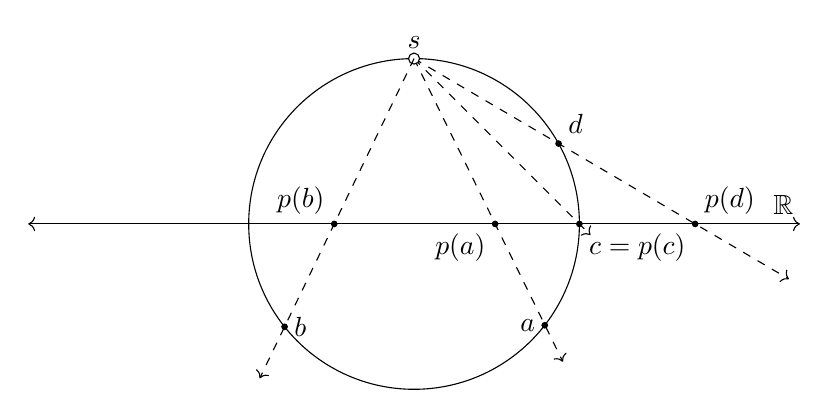
\begin{tikzpicture}[scale=0.7]
      \draw (0,0) circle (3);
      \node[above] at (0,3) {$s$};
      \draw[<->] (-7,0)--(7,0);
      \node[above] at (6.7,0) {$\mathbb{R}$};
      \draw[->, dashed] (0,3)--(3.2,-0.2);
      \draw[->, dashed] (0,3)--(2.7,-2.5);
      \draw[->, dashed] (0,3)--(6.8,-1);
      \draw[fill=white] (0,3) circle (0.1);
      \draw[->, dashed] (0,3)--(-2.8, -2.8);
      \draw[fill] (3,0) circle (0.05);
      \draw[fill] (-2.349,-1.866) circle (0.05);
      \draw[fill] (5.1,0) circle (0.05);
      \draw[fill] (2.622,1.458) circle (0.05);
      \draw[fill] (-1.448,0) circle (0.05);
      \draw[fill] (1.471,0) circle (0.05); 
      \draw[fill] (2.371, -1.838) circle (0.05);
      \node[left] at (2.371, -1.838) {$a$};
      \node[below left] at (1.471,0) {$p(a)$};
      \node[above left] at (-1.448,0) {$p(b)$};
      \node[right] at (-2.349,-1.866) {$b$};
      \node[above right] at (5.1,0) {$p(d)$};
      \node[above right] at (2.622,1.458) {$d$};
      \node[below right] at (3,0) {$c = p(c)$};
    \end{tikzpicture}
    \end{center}
    \end{example}

    \begin{example}
    The one point-compactification of the real plane $\mathbb{R}^2$ is homeomorphic to the 2-sphere $S^2$. That is, 
    \[\mathbb{R}^2 \cup \{\infty\} \cong S^2\]
    We can similarly imagine this homeomorphism using the stereographic projection. 
    \begin{center}
        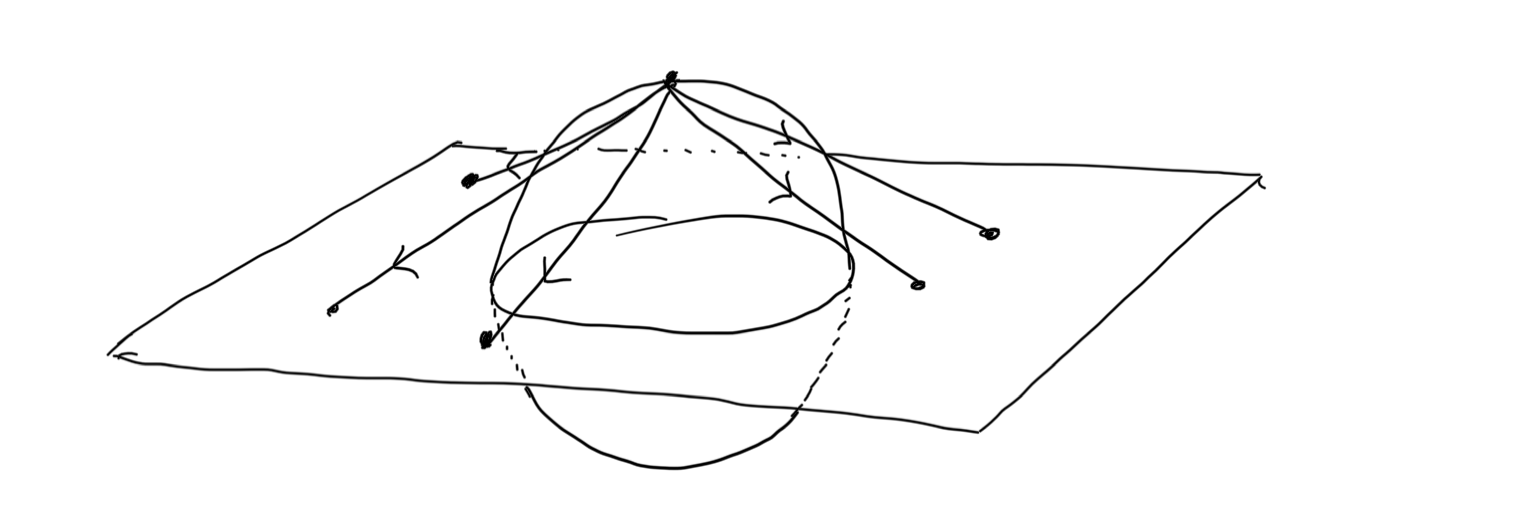
\includegraphics[scale=0.23]{img/Two_Dim_Stereographic_Projection.PNG}
    \end{center}
    \end{example}

    \begin{lemma}
    Let $X$ be a Hausdorff space. Then $X$ is locally compact at $x$ if and only if for every neighborhood $U$ of $x$, there is a neighborhood $V$ of $x$ such that $\bar{V}$ is compact and $\bar{V} \subset U$. 
    \end{lemma}

    \begin{corollary}
    Let $X$ be a locally compact Hausdorff space with $Y$ a subspace of $X$. If $Y$ is closed in $X$ or open in $X$, then $Y$ is locally compact. 
    \end{corollary}

    \begin{corollary}
    A space $X$ is homeomorphic to an open subset of a compact Hausdorff space if and only if $X$ is locally compact and Hausdorff. 
    \end{corollary}

\section{Countability and Separation Axioms}

    \begin{definition}
    A space $X$ is said to have a countable basis at $x$ if there exists a sequence $N_1, N_2, ...$ of open neighborhoods of $x$ such that for any neighborhood $N$ of $x$, there exists an integer $i$ such that $N_i \in N$. That is, the countable basis of neighborhoods get arbitrarily small around $x$. A space $X$ satisfying this axiom at every point $x \in X$ is said to be a \textbf{first-countable space}. 
    \end{definition}

    In particular, every metric space is first-countable, since we can construct the sequence of open balls $B (x, \frac{1}{n})$ for each $n \in \mathbb{N}$ which forms a countable basis at $x$. 

    We now generalize some previous statements about metric spaces to statements about first-countable spaces. 

    \begin{theorem}
    Let $X$ be a space satisfying the first countability axiom, and let $A \subset X$. 
    \begin{enumerate}
        \item $x \in \bar{A}$ if and only if there exists a sequence of points in $A$ converging to $x$. 
        \item The function $f: X \longrightarrow Y$ is continuous if and only if for every convergent sequence $(x_n) \rightarrow x$ in $X$, the sequence $\big( f(x_n)\big) \rightarrow f(x)$ in $Y$. 
    \end{enumerate}
    \end{theorem}

    \begin{definition}
    A topological space $X$ is said to satisfy the \textbf{second countability axiom} if $X$ has a countable basis for its topology.
    \end{definition}

    \begin{proposition}
    Second countability implies first countability. 
    \end{proposition}
    \begin{proof}
    If $\mathscr{B}$ is a countable basis for the topology of $X$, then the subset of $\mathscr{B}$ consisting of elements containing the point $x$ is a countable basis at $x$. 
    \end{proof}

    \begin{example}
    The real line $\mathbb{R}$ is second countable. We can contrust a countable basis as the set of all open intervals $(a, b)$ with rational end points. Likewise, $\mathbb{R}^n$ has a countable basis, which is the collection of all products of intervals having rational end points. Additionally, $\mathbb{R}^\omega$ has a countable basis. It is the collection of all products
    \[\prod_{n \in \mathbb{N}} U_n\]
    where $U_n$ is an open interval with rational endpoints for finitely many values of $n$ and $U_n = \mathbb{R}$ for all other values of $n$. 
    \end{example}

    \begin{example}
    In the uniform topology, $\mathbb{R}^\omega$ satisfies the first countability axiom (since it is metrizable). 
    \end{example}

    \begin{theorem}
    A subspace of a first and second countable space is first and second countable, respectively. A countable product of first and second countable space is first and second countable, respectively. 
    \end{theorem}

    \begin{theorem}
    A subset $A$ of space $X$ is said to be \textbf{dense} in $X$ if $\bar{A} = X$. 
    \end{theorem}

    \begin{theorem}
    Suppose that $X$ has a countable basis. Then, 
    \begin{enumerate}
        \item Every open cover of $X$ has a countable subcover. 
        \item There exists a countable subset of $X$ which is dense in $X$. 
    \end{enumerate}
    \end{theorem}
    \begin{proof}
    a) Let $\mathscr{B} = \{B_n\}_{n \in \mathbb{N}}$ be a countable basis for $X$, and let $\mathscr{A}$ be an open covering of $X$. For each integer $n \in \mathbb{N}$, chose an element $A_n \in \mathscr{A}$ containing the basis element $B_n$. The newly formed collection $\mathscr{A}^\prime$ of all the $A_n$'s is countable since it is indexed according to a subset of $\mathbb{N}$. Furthermore, since $B_n \subset A_n$ for every $B_n$ in the basis, the $A_n$ clearly covers $X$. \\
    b) From each nonempty basis element $B_n$, we choose a point $x_n$. The set 
    \[D \equiv \{x_n \; | \; n \in \mathbb{N}\}\]
    is dense in $X$, since given any $x \in X$, every open basis element $B_x$ about $x$ intersects $D$. That is, 
    \[B_x \cap D \neq \emptyset\]
    meaning that the set of points $x_n$ get arbitrarily close to $x$. 
    \end{proof}

    \begin{definition}
    A space for which every open covering contains a countable subcovering is called a \textbf{Lindelof space}. 
    \end{definition}

    \begin{definition}
    A topological space $X$ is called a \textbf{Hausdorff space} if for each pair of distinct points $p, q \in X$, there exists neighborhoods $U_p, U_q$ that are disjoint. $X$ is also said to be \textbf{$t_2$-separable.}
    \begin{center}
        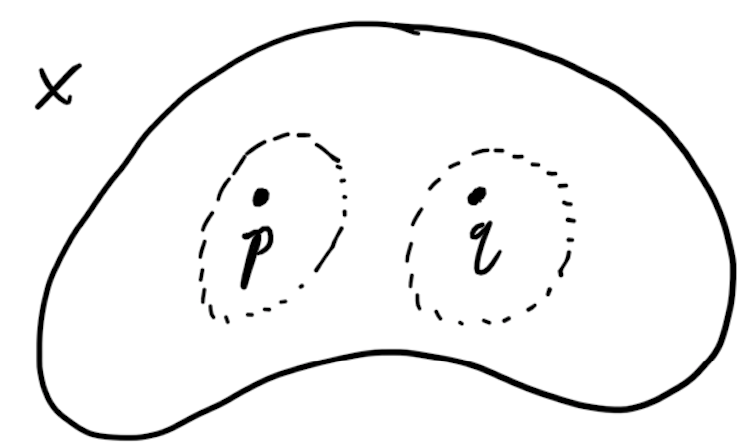
\includegraphics[scale=0.35]{img/Hausdorff_Space_Separability.PNG}
    \end{center}
    \end{definition}

    \begin{theorem}
    Every finite point set in a Hausdorff space $X$ is closed. 
    \end{theorem}
    \begin{proof}
    It suffices to show that every one point set $\{x_0\}$ is closed. If $x$ and $x_0$ are distinct points, then by definition of Hausdorff spaces they have disjoint neighborhoods $U_x$ and $U_{x_0} \implies x \not\in \bar{\{x_0\}} \implies \{x_0\} = \bar{\{x_0\}}$, so $\{x_0\}$ is closed. 
    \end{proof}

    \begin{theorem}
    Given Hausdorff space $X$ and subset $A \subset X$ a point $x$ is a limit point of $A$ if and only if every neighborhood of $x$ contains infinitely many point of $A$. 
    \end{theorem}
    \begin{proof}
    $(\rightarrow)$ Assume that $x$ is a limit point of $A$ with some neighborhood $U_x$ intersecting $A$ in finitely many points. Then, let the points of intersections be 
    \[\{x_1, ..., x_n\} = A \cap \{U_x \setminus \{x\} \} \]
    But $U_x \setminus \{x\}$ is open $\implies H \equiv \{U_x \setminus ( \{x\} \cup \{x_1, ..., x_n\})\}$ is open. But $H \cap A = \emptyset$, contradicting the assumption that $x$ is a limit point. \\
    $(\leftarrow)$ Simple. 
    \end{proof}

    \begin{theorem}
    The product of 2 Hausdorff spaces is Hausdorff. A subspace of a Hausdorff space is a Hausdorff space. 
    \end{theorem}

    Generally, mathematicians consider the Hausdorff condition as a mild extra conditions on topological spaces that make it much easier to deal with. We will assume that most of the topological spaces we work with are Hausdorff. 


    \begin{definition}
    Suppose that one-point sets are closed in $X$. Then, $X$ is said to be \textbf{regular} if for each pair consisting of a point $x$ and a closed set $B$ disjoint from $x$, there exist disjoint open sets containing $x$ and $B$, respectively. $X$ is also said to be $t_3$-separable. 
    \end{definition}

    \begin{definition}
    The space $X$ is said to be \textbf{normal} if for each pair $A, B$ of disjoint closed sets of $X$, there exist disjoint open sets containing $A$ and $B$, respectively. $X$ is also said to be $t_4$-separable. 
    \end{definition}

    \begin{lemma}
    Let $X$ be a topological space. Let one-point sets in $X$ be closed. 
    \begin{enumerate}
        \item $X$ is regular if and only if given a point $x \in X$ and a neighborhood $U$ of $x$, there is a neighborhood $V$ of $x$ such that $\bar{V} \subset U$. 
        \item $X$ is normal if and only if given a closed set $A$ and an open set $U$ containing $A$, there exists an open set $V$ containing $A$ such that $\bar{V} \subset U$. 
    \end{enumerate}
    \end{lemma}

    \begin{theorem}
    \begin{enumerate}
        \item A subspace of a Hausdorff space is Hausdorff; a product of Hausdorff spaces is Hausdorff. 
        \item A subspace of a regular space is regular; a product of regular spaces is regular. 
        \item However, a subspace of a normal space is not necessarily normal; a product of normal spaces is not necessarily normal. 
    \end{enumerate}
    \end{theorem}

    \begin{theorem}
    Every metrizable space is normal. 
    \end{theorem}

    \begin{theorem}
    Every compact Hausdorff space is normal. 
    \end{theorem}

    \begin{theorem}
    Every regular space with a countable basis is normal. 
    \end{theorem}

    \begin{theorem}
    Every well-ordered set $X$ is normal in the order topology. 
    \end{theorem}

  \subsection{The Urysohn Lemma}

    \begin{theorem}[Urysohn Lemma]
    Let $X$ be a normal space, and let $A, B$ be disjoint closed subsets of $X$. Let $[a,b]$ be a closed interval in the real line. Then there exists a continuous map
    \[f: X \longrightarrow [a,b]\]
    such that $f(x) = a$ for every $x \in A$ and $f(x) = b$ for every $x \in B$. 
    \end{theorem}


    \begin{definition}
    If $A$ and $B$ are two subsets of the topological space $X$, and if there is a continuous function $f: X \longrightarrow [0,1]$ such that $f(A) = \{0\}$ and $f(B) = \{1\}$, it is said that \textbf{$A$ and $B$ can be separated by a continuous function}. 
    \end{definition}

    More colloquially, the lemma states that if every pair of disjoint closed sets in $X$ can be separated by disjoint open sets, then each such pair can be separated by a continuous function. 

    \begin{theorem}[Tietze Extension Theorem]
    Let $X$ be a normal space and let $A$ be a closed subset of $X$. 
    \begin{enumerate}
        \item Any continuous map of $A$ into the closed interval $[a,b] \subset \mathbb{R}$ may be extended to a continuous map of all $X$ into $[a,b]$. 
        \item Any continuous map $A$ into the reals $\mathbb{R}$ may be extended to a continuous map of all of $X$ into $\mathbb{R}$. 
    \end{enumerate}
    \end{theorem}

  \subsection{The Urysohn Metrization Theorem}

    \begin{theorem}[Urysohn Metrization Theorem]
    Every regular space $X$ with a countable basis is metrizable. 
    \end{theorem}

    \begin{theorem}[Imbedding Theorem]
    Let $X$ be Hausdorff. Suppose that 
    \[\{f_\alpha\}_{\alpha \in J}, \; f_\alpha: X \longrightarrow \mathbb{R}\]
    is a collection of continuous functions satisfying the requirement that for each point $x_0 \in X$ and each neighborhood $U$ of $x_0$, there is an index $\alpha$ such that $f_\alpha$ is positive at $x_0$ and vanishes outside $U$. Then, the function 
    \[F: X \longrightarrow \mathbb{R}^J, \; F(x) \equiv \big( f_\alpha (x)\big)_{\alpha \in J}\]
    is an \textbf{imbedding} of $X$ in $\mathbb{R}^J$.
    \end{theorem}

\section{The Tychonoff Theorem}

  \begin{theorem}
  An arbitrary product of compact spaces is compact under the product topology. 
  \end{theorem}

  \begin{definition}
  A space $X$ is \textbf{completely regular} if one-point sets are closed in $X$ and if for each point $x_0$ and each closed set $A$ not containing $x_0$, there is a continuous function $f: X \longrightarrow [0,1]$ such that $f(x_0) = 1$ and $f(A) = \{0\}$. 
  \end{definition}

  \begin{theorem}
  A subspace of a completely regular space is completely regular. A product of completely regular spaces is completely regular. 
  \end{theorem}

  \begin{theorem}
  If $X$ is completely regular, then $X$ can be imbedded in $[0,1]^J$ for some $J$. 
  \end{theorem}

  \begin{corollary}
  Let $X$ be a space. The following are equivalent: 
  \begin{enumerate}
      \item $X$ is completely regular. 
      \item $X$ is homeomorphic to a subspace of a compact Hausdorff space. 
      \item $X$ is homeomorphic to a subspace of a normal space. 
  \end{enumerate}
  \end{corollary}

  \begin{definition}
  A \textbf{compactification} of a space $X$ is a compact Hausdorff space $Y$ containing $X$ such that $X$ is dense in $Y$ (that is $\bar{X} = Y$). Two compactifications $Y_1$ and $Y_2$ of $X$ are said to be \textbf{equivalent} if there is a homeomorphism $h: Y_1 \longrightarrow Y_2$ such that $h(x) = x$ for every $x \in X$. 
  \end{definition}

  \begin{theorem}
  Let $X$ be completely regular, and let $\beta(X)$ be its Stone-Cech compatification. Then every bounded continuous real-valued function on $X$ can be uniquely extended to a continuous real-valued function on $\beta(X)$. 
  \end{theorem}

  \begin{lemma}
  Let $A \subset X$, and let $f: A \longrightarrow Z$ be a continuous map of $A$ into the Hausdorff space $Z$. There is at most one extension of $f$ to a continuous function $g: \bar{A} \longrightarrow Z$. 
  \end{lemma}

  \begin{theorem}
  Let $X$ be completely regular. Let $Y_1, Y_2$ be two compactifications of $X$ having the extension property. Then there is a homeomorphism $\phi$ of $Y_1$ onto $Y_2$ such that $\phi(x) = x$ for each $x \in X$. 
  \end{theorem}

\end{document}
